\documentclass[twoside]{book}

% Packages required by doxygen
\usepackage{fixltx2e}
\usepackage{calc}
\usepackage{doxygen}
\usepackage[export]{adjustbox} % also loads graphicx
\usepackage{graphicx}
\usepackage[utf8]{inputenc}
\usepackage{makeidx}
\usepackage{multicol}
\usepackage{multirow}
\PassOptionsToPackage{warn}{textcomp}
\usepackage{textcomp}
\usepackage[nointegrals]{wasysym}
\usepackage[table]{xcolor}

% Font selection
\usepackage[T1]{fontenc}
\usepackage[scaled=.90]{helvet}
\usepackage{courier}
\usepackage{amssymb}
\usepackage{sectsty}
\renewcommand{\familydefault}{\sfdefault}
\allsectionsfont{%
  \fontseries{bc}\selectfont%
  \color{darkgray}%
}
\renewcommand{\DoxyLabelFont}{%
  \fontseries{bc}\selectfont%
  \color{darkgray}%
}
\newcommand{\+}{\discretionary{\mbox{\scriptsize$\hookleftarrow$}}{}{}}

% Page & text layout
\usepackage{geometry}
\geometry{%
  a4paper,%
  top=2.5cm,%
  bottom=2.5cm,%
  left=2.5cm,%
  right=2.5cm%
}
\tolerance=750
\hfuzz=15pt
\hbadness=750
\setlength{\emergencystretch}{15pt}
\setlength{\parindent}{0cm}
\setlength{\parskip}{3ex plus 2ex minus 2ex}
\makeatletter
\renewcommand{\paragraph}{%
  \@startsection{paragraph}{4}{0ex}{-1.0ex}{1.0ex}{%
    \normalfont\normalsize\bfseries\SS@parafont%
  }%
}
\renewcommand{\subparagraph}{%
  \@startsection{subparagraph}{5}{0ex}{-1.0ex}{1.0ex}{%
    \normalfont\normalsize\bfseries\SS@subparafont%
  }%
}
\makeatother

% Headers & footers
\usepackage{fancyhdr}
\pagestyle{fancyplain}
\fancyhead[LE]{\fancyplain{}{\bfseries\thepage}}
\fancyhead[CE]{\fancyplain{}{}}
\fancyhead[RE]{\fancyplain{}{\bfseries\leftmark}}
\fancyhead[LO]{\fancyplain{}{\bfseries\rightmark}}
\fancyhead[CO]{\fancyplain{}{}}
\fancyhead[RO]{\fancyplain{}{\bfseries\thepage}}
\fancyfoot[LE]{\fancyplain{}{}}
\fancyfoot[CE]{\fancyplain{}{}}
\fancyfoot[RE]{\fancyplain{}{\bfseries\scriptsize Generated by Doxygen }}
\fancyfoot[LO]{\fancyplain{}{\bfseries\scriptsize Generated by Doxygen }}
\fancyfoot[CO]{\fancyplain{}{}}
\fancyfoot[RO]{\fancyplain{}{}}
\renewcommand{\footrulewidth}{0.4pt}
\renewcommand{\chaptermark}[1]{%
  \markboth{#1}{}%
}
\renewcommand{\sectionmark}[1]{%
  \markright{\thesection\ #1}%
}

% Indices & bibliography
\usepackage{natbib}
\usepackage[titles]{tocloft}
\setcounter{tocdepth}{3}
\setcounter{secnumdepth}{5}
\makeindex

% Hyperlinks (required, but should be loaded last)
\usepackage{ifpdf}
\ifpdf
  \usepackage[pdftex,pagebackref=true]{hyperref}
\else
  \usepackage[ps2pdf,pagebackref=true]{hyperref}
\fi
\hypersetup{%
  colorlinks=true,%
  linkcolor=blue,%
  citecolor=blue,%
  unicode%
}

% Custom commands
\newcommand{\clearemptydoublepage}{%
  \newpage{\pagestyle{empty}\cleardoublepage}%
}

\usepackage{caption}
\captionsetup{labelsep=space,justification=centering,font={bf},singlelinecheck=off,skip=4pt,position=top}

%===== C O N T E N T S =====

\begin{document}

% Titlepage & ToC
\hypersetup{pageanchor=false,
             bookmarksnumbered=true,
             pdfencoding=unicode
            }
\pagenumbering{roman}
\begin{titlepage}
\vspace*{7cm}
\begin{center}%
{\Large Juego de la vida }\\
\vspace*{1cm}
{\large Generated by Doxygen 1.8.11}\\
\end{center}
\end{titlepage}
\clearemptydoublepage
\tableofcontents
\clearemptydoublepage
\pagenumbering{arabic}
\hypersetup{pageanchor=true}

%--- Begin generated contents ---
\chapter{Hierarchical Index}
\section{Class Hierarchy}
This inheritance list is sorted roughly, but not completely, alphabetically\+:\begin{DoxyCompactList}
\item \contentsline{section}{Animal}{\pageref{classAnimal}}{}
\begin{DoxyCompactList}
\item \contentsline{section}{Lobo}{\pageref{classLobo}}{}
\item \contentsline{section}{Oveja}{\pageref{classOveja}}{}
\item \contentsline{section}{Raton}{\pageref{classRaton}}{}
\item \contentsline{section}{Zorro}{\pageref{classZorro}}{}
\end{DoxyCompactList}
\item \contentsline{section}{Celda}{\pageref{classCelda}}{}
\item \contentsline{section}{Controlador}{\pageref{classControlador}}{}
\end{DoxyCompactList}

\chapter{Class Index}
\section{Data Structures}
Here are the data structures with brief descriptions\+:\begin{DoxyCompactList}
\item\contentsline{section}{\hyperlink{classBPlusTree}{B\+Plus\+Tree$<$ Data $>$} }{\pageref{classBPlusTree}}{}
\item\contentsline{section}{\hyperlink{classLeaf}{Leaf$<$ Data $>$} }{\pageref{classLeaf}}{}
\item\contentsline{section}{\hyperlink{classNode}{Node$<$ Data $>$} }{\pageref{classNode}}{}
\end{DoxyCompactList}

\chapter{File Index}
\section{File List}
Here is a list of all files with brief descriptions\+:\begin{DoxyCompactList}
\item\contentsline{section}{\hyperlink{BPlusTree_8h}{B\+Plus\+Tree.\+h} }{\pageref{BPlusTree_8h}}{}
\item\contentsline{section}{\hyperlink{Leaf_8h}{Leaf.\+h} }{\pageref{Leaf_8h}}{}
\item\contentsline{section}{\hyperlink{main_8cpp}{main.\+cpp} }{\pageref{main_8cpp}}{}
\item\contentsline{section}{\hyperlink{Node_8h}{Node.\+h} \\*Clase Arbol\+B+ }{\pageref{Node_8h}}{}
\end{DoxyCompactList}

\chapter{Class Documentation}
\hypertarget{classAnimal}{}\section{Animal Class Reference}
\label{classAnimal}\index{Animal@{Animal}}


{\ttfamily \#include $<$Animal.\+h$>$}



Inheritance diagram for Animal\+:\nopagebreak
\begin{figure}[H]
\begin{center}
\leavevmode
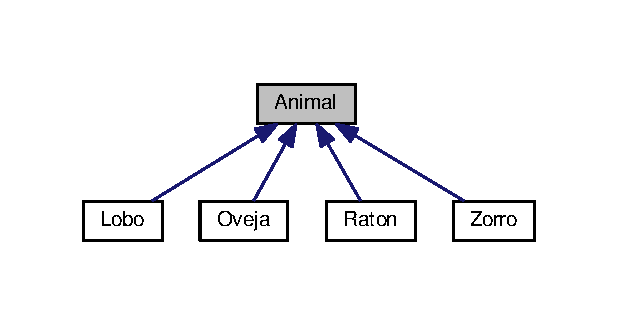
\includegraphics[width=350pt]{classAnimal__inherit__graph}
\end{center}
\end{figure}


Collaboration diagram for Animal\+:\nopagebreak
\begin{figure}[H]
\begin{center}
\leavevmode
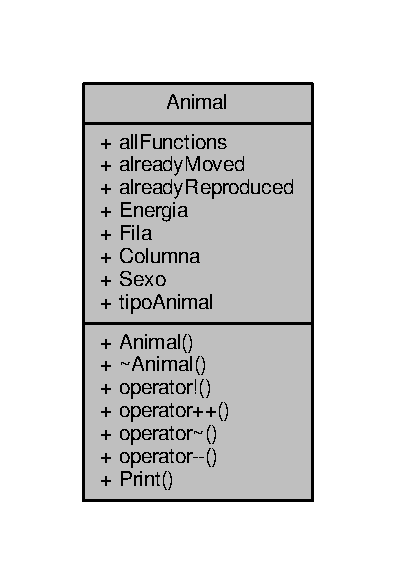
\includegraphics[width=190pt]{classAnimal__coll__graph}
\end{center}
\end{figure}
\subsection*{Public Member Functions}
\begin{DoxyCompactItemize}
\item 
\hyperlink{classAnimal_a1e726a49ec952443190ac62dad22353c}{Animal} ()
\begin{DoxyCompactList}\small\item\em Constructor por defecto. \end{DoxyCompactList}\item 
virtual \hyperlink{classAnimal_a476af25adde5f0dfa688129c8f86fa5c}{$\sim$\+Animal} ()
\begin{DoxyCompactList}\small\item\em Destructor. \end{DoxyCompactList}\item 
virtual int \hyperlink{classAnimal_abe502d1333df77d245d74cd20190a0aa}{operator!} ()=0
\item 
virtual int \hyperlink{classAnimal_a66e3bc83959ea5c5d7aa8d85f8ca993c}{operator++} ()=0
\item 
virtual void \hyperlink{classAnimal_a6539ec18d8975982b65de76d8e5638f0}{operator$\sim$} ()=0
\item 
bool \hyperlink{classAnimal_a7c407c852d55806aa10b2db5844f683d}{operator-\/-\/} ()
\begin{DoxyCompactList}\small\item\em Metodo para determinar si un animal debe morir. \end{DoxyCompactList}\item 
void \hyperlink{classAnimal_aa03d8b2c76ee132f3347e7c1323d1473}{Print} ()
\begin{DoxyCompactList}\small\item\em Esta funcion se llama dentro de la funcion imprimir de celda ya que un atributo de una celda es un animal. \end{DoxyCompactList}\end{DoxyCompactItemize}
\subsection*{Public Attributes}
\begin{DoxyCompactItemize}
\item 
bool \hyperlink{classAnimal_ad014642901894565334b8d2bf3713755}{all\+Functions}
\begin{DoxyCompactList}\small\item\em Bandera para saber si a un animal ya se le aplicaron todos los metodos. \end{DoxyCompactList}\item 
bool \hyperlink{classAnimal_a1cc0126c23d1245a1f964ce636552bba}{already\+Moved}
\begin{DoxyCompactList}\small\item\em Bandera para saber si un animal ya se movio en un dia. \end{DoxyCompactList}\item 
bool \hyperlink{classAnimal_ab08fe103b56326ac66c63b0f38585c4c}{already\+Reproduced}
\begin{DoxyCompactList}\small\item\em Bandera para saber si un animal ya se repdodujo en un dia. \end{DoxyCompactList}\item 
int \hyperlink{classAnimal_af1c30573e35f61baa10094579c5e741a}{Energia}
\begin{DoxyCompactList}\small\item\em Energia del aimal. \end{DoxyCompactList}\item 
int \hyperlink{classAnimal_ab403adfd13b57143eff123bdd6a2febb}{Fila}
\begin{DoxyCompactList}\small\item\em Posicion del animal. \end{DoxyCompactList}\item 
int \hyperlink{classAnimal_a340d64e6e4ffe5f35e0855c63aad1bd3}{Columna}
\item 
int \hyperlink{classAnimal_a42b629ae5a7e0c05263a3f6e592ea116}{Sexo}
\begin{DoxyCompactList}\small\item\em Sexo del animal. \end{DoxyCompactList}\item 
string \hyperlink{classAnimal_ae7a4f121949d20c359414a3002e7eff7}{tipo\+Animal}
\begin{DoxyCompactList}\small\item\em Se define en las clases hijo, dependiendo de que tipo de animal que sea. \end{DoxyCompactList}\end{DoxyCompactItemize}


\subsection{Constructor \& Destructor Documentation}
\index{Animal@{Animal}!Animal@{Animal}}
\index{Animal@{Animal}!Animal@{Animal}}
\subsubsection[{\texorpdfstring{Animal()}{Animal()}}]{\setlength{\rightskip}{0pt plus 5cm}Animal\+::\+Animal (
\begin{DoxyParamCaption}
{}
\end{DoxyParamCaption}
)}\hypertarget{classAnimal_a1e726a49ec952443190ac62dad22353c}{}\label{classAnimal_a1e726a49ec952443190ac62dad22353c}


Constructor por defecto. 

\index{Animal@{Animal}!````~Animal@{$\sim$\+Animal}}
\index{````~Animal@{$\sim$\+Animal}!Animal@{Animal}}
\subsubsection[{\texorpdfstring{$\sim$\+Animal()}{~Animal()}}]{\setlength{\rightskip}{0pt plus 5cm}Animal\+::$\sim$\+Animal (
\begin{DoxyParamCaption}
{}
\end{DoxyParamCaption}
)\hspace{0.3cm}{\ttfamily [virtual]}}\hypertarget{classAnimal_a476af25adde5f0dfa688129c8f86fa5c}{}\label{classAnimal_a476af25adde5f0dfa688129c8f86fa5c}


Destructor. 



\subsection{Member Function Documentation}
\index{Animal@{Animal}!operator"!@{operator"!}}
\index{operator"!@{operator"!}!Animal@{Animal}}
\subsubsection[{\texorpdfstring{operator"!()=0}{operator!()=0}}]{\setlength{\rightskip}{0pt plus 5cm}virtual int Animal\+::operator! (
\begin{DoxyParamCaption}
{}
\end{DoxyParamCaption}
)\hspace{0.3cm}{\ttfamily [pure virtual]}}\hypertarget{classAnimal_abe502d1333df77d245d74cd20190a0aa}{}\label{classAnimal_abe502d1333df77d245d74cd20190a0aa}


Implemented in \hyperlink{classLobo_aba92fb0575e359e2d66134ab5754ab0d}{Lobo}, \hyperlink{classZorro_ad9d441234c592f01f5be69415d904423}{Zorro}, \hyperlink{classOveja_a408a0da02f53481fa59dc592b5b60b6e}{Oveja}, and \hyperlink{classRaton_ad50cebe48f49dbadef570d616a0e6aa3}{Raton}.

\index{Animal@{Animal}!operator++@{operator++}}
\index{operator++@{operator++}!Animal@{Animal}}
\subsubsection[{\texorpdfstring{operator++()=0}{operator++()=0}}]{\setlength{\rightskip}{0pt plus 5cm}virtual int Animal\+::operator++ (
\begin{DoxyParamCaption}
{}
\end{DoxyParamCaption}
)\hspace{0.3cm}{\ttfamily [pure virtual]}}\hypertarget{classAnimal_a66e3bc83959ea5c5d7aa8d85f8ca993c}{}\label{classAnimal_a66e3bc83959ea5c5d7aa8d85f8ca993c}


Implemented in \hyperlink{classLobo_aa7387ef43eab75b348d85c142f74b2d3}{Lobo}, \hyperlink{classZorro_ac9a48ca08f8d7f6481be2cf0115cc209}{Zorro}, \hyperlink{classOveja_a6faad614b717d9c5ad92e7787fee5419}{Oveja}, and \hyperlink{classRaton_a64ec37f911376e16802ad5906bb4e27a}{Raton}.

\index{Animal@{Animal}!operator-\/-\/@{operator-\/-\/}}
\index{operator-\/-\/@{operator-\/-\/}!Animal@{Animal}}
\subsubsection[{\texorpdfstring{operator-\/-\/()}{operator--()}}]{\setlength{\rightskip}{0pt plus 5cm}bool Animal\+::operator-\/-\/ (
\begin{DoxyParamCaption}
{}
\end{DoxyParamCaption}
)}\hypertarget{classAnimal_a7c407c852d55806aa10b2db5844f683d}{}\label{classAnimal_a7c407c852d55806aa10b2db5844f683d}


Metodo para determinar si un animal debe morir. 

\index{Animal@{Animal}!operator````~@{operator$\sim$}}
\index{operator````~@{operator$\sim$}!Animal@{Animal}}
\subsubsection[{\texorpdfstring{operator$\sim$()=0}{operator~()=0}}]{\setlength{\rightskip}{0pt plus 5cm}virtual void Animal\+::operator$\sim$ (
\begin{DoxyParamCaption}
{}
\end{DoxyParamCaption}
)\hspace{0.3cm}{\ttfamily [pure virtual]}}\hypertarget{classAnimal_a6539ec18d8975982b65de76d8e5638f0}{}\label{classAnimal_a6539ec18d8975982b65de76d8e5638f0}


Implemented in \hyperlink{classLobo_a2b4bba4b6d6efa24af4d8e3b986dc7f2}{Lobo}, \hyperlink{classZorro_a9fdef26a109d506ac85b739c9920cc85}{Zorro}, \hyperlink{classOveja_a0ff5ac43f8a666b3b130de88da605fe2}{Oveja}, and \hyperlink{classRaton_a7ec71ea95a98d13bf2cccf108b3c76d6}{Raton}.

\index{Animal@{Animal}!Print@{Print}}
\index{Print@{Print}!Animal@{Animal}}
\subsubsection[{\texorpdfstring{Print()}{Print()}}]{\setlength{\rightskip}{0pt plus 5cm}void Animal\+::\+Print (
\begin{DoxyParamCaption}
{}
\end{DoxyParamCaption}
)}\hypertarget{classAnimal_aa03d8b2c76ee132f3347e7c1323d1473}{}\label{classAnimal_aa03d8b2c76ee132f3347e7c1323d1473}


Esta funcion se llama dentro de la funcion imprimir de celda ya que un atributo de una celda es un animal. 



\subsection{Member Data Documentation}
\index{Animal@{Animal}!all\+Functions@{all\+Functions}}
\index{all\+Functions@{all\+Functions}!Animal@{Animal}}
\subsubsection[{\texorpdfstring{all\+Functions}{allFunctions}}]{\setlength{\rightskip}{0pt plus 5cm}bool Animal\+::all\+Functions}\hypertarget{classAnimal_ad014642901894565334b8d2bf3713755}{}\label{classAnimal_ad014642901894565334b8d2bf3713755}


Bandera para saber si a un animal ya se le aplicaron todos los metodos. 

\index{Animal@{Animal}!already\+Moved@{already\+Moved}}
\index{already\+Moved@{already\+Moved}!Animal@{Animal}}
\subsubsection[{\texorpdfstring{already\+Moved}{alreadyMoved}}]{\setlength{\rightskip}{0pt plus 5cm}bool Animal\+::already\+Moved}\hypertarget{classAnimal_a1cc0126c23d1245a1f964ce636552bba}{}\label{classAnimal_a1cc0126c23d1245a1f964ce636552bba}


Bandera para saber si un animal ya se movio en un dia. 

\index{Animal@{Animal}!already\+Reproduced@{already\+Reproduced}}
\index{already\+Reproduced@{already\+Reproduced}!Animal@{Animal}}
\subsubsection[{\texorpdfstring{already\+Reproduced}{alreadyReproduced}}]{\setlength{\rightskip}{0pt plus 5cm}bool Animal\+::already\+Reproduced}\hypertarget{classAnimal_ab08fe103b56326ac66c63b0f38585c4c}{}\label{classAnimal_ab08fe103b56326ac66c63b0f38585c4c}


Bandera para saber si un animal ya se repdodujo en un dia. 

\index{Animal@{Animal}!Columna@{Columna}}
\index{Columna@{Columna}!Animal@{Animal}}
\subsubsection[{\texorpdfstring{Columna}{Columna}}]{\setlength{\rightskip}{0pt plus 5cm}int Animal\+::\+Columna}\hypertarget{classAnimal_a340d64e6e4ffe5f35e0855c63aad1bd3}{}\label{classAnimal_a340d64e6e4ffe5f35e0855c63aad1bd3}
\index{Animal@{Animal}!Energia@{Energia}}
\index{Energia@{Energia}!Animal@{Animal}}
\subsubsection[{\texorpdfstring{Energia}{Energia}}]{\setlength{\rightskip}{0pt plus 5cm}int Animal\+::\+Energia}\hypertarget{classAnimal_af1c30573e35f61baa10094579c5e741a}{}\label{classAnimal_af1c30573e35f61baa10094579c5e741a}


Energia del aimal. 

\index{Animal@{Animal}!Fila@{Fila}}
\index{Fila@{Fila}!Animal@{Animal}}
\subsubsection[{\texorpdfstring{Fila}{Fila}}]{\setlength{\rightskip}{0pt plus 5cm}int Animal\+::\+Fila}\hypertarget{classAnimal_ab403adfd13b57143eff123bdd6a2febb}{}\label{classAnimal_ab403adfd13b57143eff123bdd6a2febb}


Posicion del animal. 

\index{Animal@{Animal}!Sexo@{Sexo}}
\index{Sexo@{Sexo}!Animal@{Animal}}
\subsubsection[{\texorpdfstring{Sexo}{Sexo}}]{\setlength{\rightskip}{0pt plus 5cm}int Animal\+::\+Sexo}\hypertarget{classAnimal_a42b629ae5a7e0c05263a3f6e592ea116}{}\label{classAnimal_a42b629ae5a7e0c05263a3f6e592ea116}


Sexo del animal. 

\index{Animal@{Animal}!tipo\+Animal@{tipo\+Animal}}
\index{tipo\+Animal@{tipo\+Animal}!Animal@{Animal}}
\subsubsection[{\texorpdfstring{tipo\+Animal}{tipoAnimal}}]{\setlength{\rightskip}{0pt plus 5cm}string Animal\+::tipo\+Animal}\hypertarget{classAnimal_ae7a4f121949d20c359414a3002e7eff7}{}\label{classAnimal_ae7a4f121949d20c359414a3002e7eff7}


Se define en las clases hijo, dependiendo de que tipo de animal que sea. 



The documentation for this class was generated from the following files\+:\begin{DoxyCompactItemize}
\item 
\hyperlink{Animal_8h}{Animal.\+h}\item 
\hyperlink{Animal_8cpp}{Animal.\+cpp}\end{DoxyCompactItemize}

\hypertarget{classCelda}{}\section{Celda Class Reference}
\label{classCelda}\index{Celda@{Celda}}


{\ttfamily \#include $<$Celda.\+h$>$}



Collaboration diagram for Celda\+:
\nopagebreak
\begin{figure}[H]
\begin{center}
\leavevmode
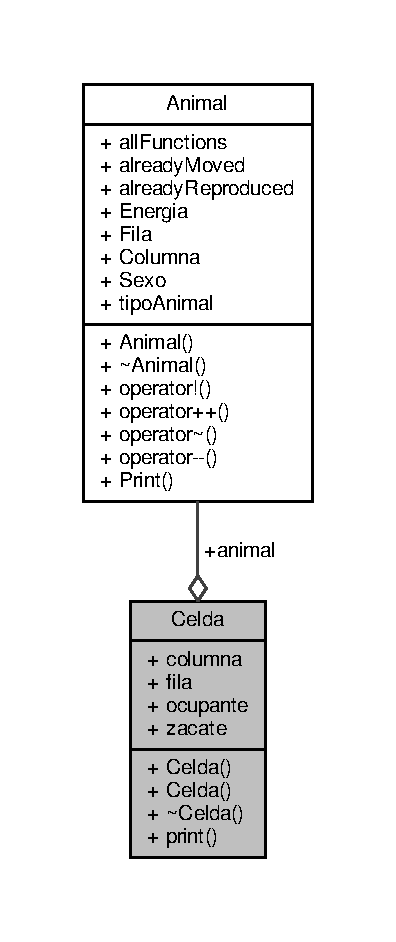
\includegraphics[width=136pt]{classCelda__coll__graph}
\end{center}
\end{figure}
\subsection*{Public Member Functions}
\begin{DoxyCompactItemize}
\item 
\hyperlink{classCelda_af1dadd95735043294599490d4abc6dc1}{Celda} ()
\begin{DoxyCompactList}\small\item\em Constructor por defecto. \end{DoxyCompactList}\item 
\hyperlink{classCelda_a03a6dc5cb3f51bc24efcc8d00e797d32}{Celda} (int cantidad\+Zacate, string tipo\+Ocupante, int \hyperlink{classCelda_a5f93fabd067087b5679e6226c7eb4313}{columna}, int \hyperlink{classCelda_a58bd35cc52cc550b75a33cdaccdd014b}{fila})
\begin{DoxyCompactList}\small\item\em Constructor para crear \hyperlink{classCelda}{Celda} con datos especificos. \end{DoxyCompactList}\item 
virtual \hyperlink{classCelda_a256de3b5c647bbbe404e4b40aca0d0f2}{$\sim$\+Celda} ()
\begin{DoxyCompactList}\small\item\em Destructor. \end{DoxyCompactList}\item 
void \hyperlink{classCelda_a915164163bf22fd3277d7791074d8bbe}{print} ()
\begin{DoxyCompactList}\small\item\em Se imprime toda la informacion relevane de una celda y de el animal que esta dentro de ella. \end{DoxyCompactList}\end{DoxyCompactItemize}
\subsection*{Data Fields}
\begin{DoxyCompactItemize}
\item 
\hyperlink{classAnimal}{Animal} $\ast$ \hyperlink{classCelda_a57f99719090f3f2cc587ca5ea89d6f7d}{animal}
\begin{DoxyCompactList}\small\item\em \hyperlink{classAnimal}{Animal} que se encuetra en la celda. \end{DoxyCompactList}\item 
int \hyperlink{classCelda_a5f93fabd067087b5679e6226c7eb4313}{columna}
\begin{DoxyCompactList}\small\item\em Posicion de la celda. \end{DoxyCompactList}\item 
int \hyperlink{classCelda_a58bd35cc52cc550b75a33cdaccdd014b}{fila}
\item 
string \hyperlink{classCelda_aa9893b7aca0260a6305a8756971c1a53}{ocupante}
\begin{DoxyCompactList}\small\item\em Tipo de animal que ocupa la celda. \end{DoxyCompactList}\item 
int \hyperlink{classCelda_ad5e9456beab1d6fbe306642fe7198043}{zacate}
\begin{DoxyCompactList}\small\item\em Cantidad de zacate presente en la celda. \end{DoxyCompactList}\end{DoxyCompactItemize}


\subsection{Constructor \& Destructor Documentation}
\index{Celda@{Celda}!Celda@{Celda}}
\index{Celda@{Celda}!Celda@{Celda}}
\subsubsection[{\texorpdfstring{Celda()}{Celda()}}]{\setlength{\rightskip}{0pt plus 5cm}Celda\+::\+Celda (
\begin{DoxyParamCaption}
{}
\end{DoxyParamCaption}
)}\hypertarget{classCelda_af1dadd95735043294599490d4abc6dc1}{}\label{classCelda_af1dadd95735043294599490d4abc6dc1}


Constructor por defecto. 

\index{Celda@{Celda}!Celda@{Celda}}
\index{Celda@{Celda}!Celda@{Celda}}
\subsubsection[{\texorpdfstring{Celda(int cantidad\+Zacate, string tipo\+Ocupante, int columna, int fila)}{Celda(int cantidadZacate, string tipoOcupante, int columna, int fila)}}]{\setlength{\rightskip}{0pt plus 5cm}Celda\+::\+Celda (
\begin{DoxyParamCaption}
\item[{int}]{cantidad\+Zacate, }
\item[{string}]{tipo\+Ocupante, }
\item[{int}]{columna, }
\item[{int}]{fila}
\end{DoxyParamCaption}
)}\hypertarget{classCelda_a03a6dc5cb3f51bc24efcc8d00e797d32}{}\label{classCelda_a03a6dc5cb3f51bc24efcc8d00e797d32}


Constructor para crear \hyperlink{classCelda}{Celda} con datos especificos. 

\index{Celda@{Celda}!````~Celda@{$\sim$\+Celda}}
\index{````~Celda@{$\sim$\+Celda}!Celda@{Celda}}
\subsubsection[{\texorpdfstring{$\sim$\+Celda()}{~Celda()}}]{\setlength{\rightskip}{0pt plus 5cm}Celda\+::$\sim$\+Celda (
\begin{DoxyParamCaption}
{}
\end{DoxyParamCaption}
)\hspace{0.3cm}{\ttfamily [virtual]}}\hypertarget{classCelda_a256de3b5c647bbbe404e4b40aca0d0f2}{}\label{classCelda_a256de3b5c647bbbe404e4b40aca0d0f2}


Destructor. 



\subsection{Member Function Documentation}
\index{Celda@{Celda}!print@{print}}
\index{print@{print}!Celda@{Celda}}
\subsubsection[{\texorpdfstring{print()}{print()}}]{\setlength{\rightskip}{0pt plus 5cm}void Celda\+::print (
\begin{DoxyParamCaption}
{}
\end{DoxyParamCaption}
)}\hypertarget{classCelda_a915164163bf22fd3277d7791074d8bbe}{}\label{classCelda_a915164163bf22fd3277d7791074d8bbe}


Se imprime toda la informacion relevane de una celda y de el animal que esta dentro de ella. 



\subsection{Field Documentation}
\index{Celda@{Celda}!animal@{animal}}
\index{animal@{animal}!Celda@{Celda}}
\subsubsection[{\texorpdfstring{animal}{animal}}]{\setlength{\rightskip}{0pt plus 5cm}{\bf Animal}$\ast$ Celda\+::animal}\hypertarget{classCelda_a57f99719090f3f2cc587ca5ea89d6f7d}{}\label{classCelda_a57f99719090f3f2cc587ca5ea89d6f7d}


\hyperlink{classAnimal}{Animal} que se encuetra en la celda. 

\index{Celda@{Celda}!columna@{columna}}
\index{columna@{columna}!Celda@{Celda}}
\subsubsection[{\texorpdfstring{columna}{columna}}]{\setlength{\rightskip}{0pt plus 5cm}int Celda\+::columna}\hypertarget{classCelda_a5f93fabd067087b5679e6226c7eb4313}{}\label{classCelda_a5f93fabd067087b5679e6226c7eb4313}


Posicion de la celda. 

\index{Celda@{Celda}!fila@{fila}}
\index{fila@{fila}!Celda@{Celda}}
\subsubsection[{\texorpdfstring{fila}{fila}}]{\setlength{\rightskip}{0pt plus 5cm}int Celda\+::fila}\hypertarget{classCelda_a58bd35cc52cc550b75a33cdaccdd014b}{}\label{classCelda_a58bd35cc52cc550b75a33cdaccdd014b}
\index{Celda@{Celda}!ocupante@{ocupante}}
\index{ocupante@{ocupante}!Celda@{Celda}}
\subsubsection[{\texorpdfstring{ocupante}{ocupante}}]{\setlength{\rightskip}{0pt plus 5cm}string Celda\+::ocupante}\hypertarget{classCelda_aa9893b7aca0260a6305a8756971c1a53}{}\label{classCelda_aa9893b7aca0260a6305a8756971c1a53}


Tipo de animal que ocupa la celda. 

\index{Celda@{Celda}!zacate@{zacate}}
\index{zacate@{zacate}!Celda@{Celda}}
\subsubsection[{\texorpdfstring{zacate}{zacate}}]{\setlength{\rightskip}{0pt plus 5cm}int Celda\+::zacate}\hypertarget{classCelda_ad5e9456beab1d6fbe306642fe7198043}{}\label{classCelda_ad5e9456beab1d6fbe306642fe7198043}


Cantidad de zacate presente en la celda. 



The documentation for this class was generated from the following files\+:\begin{DoxyCompactItemize}
\item 
\hyperlink{Celda_8h}{Celda.\+h}\item 
\hyperlink{Celda_8cpp}{Celda.\+cpp}\end{DoxyCompactItemize}

\hypertarget{classControlador}{}\section{Controlador Class Reference}
\label{classControlador}\index{Controlador@{Controlador}}


{\ttfamily \#include $<$Controlador.\+h$>$}

\subsection*{Public Member Functions}
\begin{DoxyCompactItemize}
\item 
\hyperlink{classControlador_a17db08229680461d4d1a2110a92ccf78}{Controlador} ()
\begin{DoxyCompactList}\small\item\em Constructor por defecto. \end{DoxyCompactList}\item 
virtual \hyperlink{classControlador_a2f1828135645f009d3772de86f12d507}{$\sim$\+Controlador} ()
\begin{DoxyCompactList}\small\item\em Destructor. \end{DoxyCompactList}\item 
void \hyperlink{classControlador_ae18001a1939880c3600e323ef4177e3a}{reset\+Reproduce\+Mark} (int columns, int rows, \hyperlink{classCelda}{Celda} $\ast$$\ast$$\ast$terreno)
\begin{DoxyCompactList}\small\item\em Metodo para resetear banderas de control. Cada animal tiene una marca que dice si ya se reprodujo, se movio y aplicaron demas metodos cada dia, entonces al finalizar cada dia se resetean las marcas de todos los animales para que al dia siguiente puedan ser aplicadas nuevamente. \end{DoxyCompactList}\item 
int \hyperlink{classControlador_a33ea3e8f5c32cd2fcd962da6e7fadf52}{run} (int amount\+Of\+Days, char $\ast$file\+Name)
\begin{DoxyCompactList}\small\item\em Metodo que ejecuta la logica del juego. \end{DoxyCompactList}\end{DoxyCompactItemize}


\subsection{Constructor \& Destructor Documentation}
\index{Controlador@{Controlador}!Controlador@{Controlador}}
\index{Controlador@{Controlador}!Controlador@{Controlador}}
\subsubsection[{\texorpdfstring{Controlador()}{Controlador()}}]{\setlength{\rightskip}{0pt plus 5cm}Controlador\+::\+Controlador (
\begin{DoxyParamCaption}
{}
\end{DoxyParamCaption}
)}\hypertarget{classControlador_a17db08229680461d4d1a2110a92ccf78}{}\label{classControlador_a17db08229680461d4d1a2110a92ccf78}


Constructor por defecto. 

\index{Controlador@{Controlador}!````~Controlador@{$\sim$\+Controlador}}
\index{````~Controlador@{$\sim$\+Controlador}!Controlador@{Controlador}}
\subsubsection[{\texorpdfstring{$\sim$\+Controlador()}{~Controlador()}}]{\setlength{\rightskip}{0pt plus 5cm}Controlador\+::$\sim$\+Controlador (
\begin{DoxyParamCaption}
{}
\end{DoxyParamCaption}
)\hspace{0.3cm}{\ttfamily [virtual]}}\hypertarget{classControlador_a2f1828135645f009d3772de86f12d507}{}\label{classControlador_a2f1828135645f009d3772de86f12d507}


Destructor. 



\subsection{Member Function Documentation}
\index{Controlador@{Controlador}!reset\+Reproduce\+Mark@{reset\+Reproduce\+Mark}}
\index{reset\+Reproduce\+Mark@{reset\+Reproduce\+Mark}!Controlador@{Controlador}}
\subsubsection[{\texorpdfstring{reset\+Reproduce\+Mark(int columns, int rows, Celda $\ast$$\ast$$\ast$terreno)}{resetReproduceMark(int columns, int rows, Celda ***terreno)}}]{\setlength{\rightskip}{0pt plus 5cm}void Controlador\+::reset\+Reproduce\+Mark (
\begin{DoxyParamCaption}
\item[{int}]{columns, }
\item[{int}]{rows, }
\item[{{\bf Celda} $\ast$$\ast$$\ast$}]{terreno}
\end{DoxyParamCaption}
)}\hypertarget{classControlador_ae18001a1939880c3600e323ef4177e3a}{}\label{classControlador_ae18001a1939880c3600e323ef4177e3a}


Metodo para resetear banderas de control. Cada animal tiene una marca que dice si ya se reprodujo, se movio y aplicaron demas metodos cada dia, entonces al finalizar cada dia se resetean las marcas de todos los animales para que al dia siguiente puedan ser aplicadas nuevamente. 

\index{Controlador@{Controlador}!run@{run}}
\index{run@{run}!Controlador@{Controlador}}
\subsubsection[{\texorpdfstring{run(int amount\+Of\+Days, char $\ast$file\+Name)}{run(int amountOfDays, char *fileName)}}]{\setlength{\rightskip}{0pt plus 5cm}int Controlador\+::run (
\begin{DoxyParamCaption}
\item[{int}]{amount\+Of\+Days, }
\item[{char $\ast$}]{file\+Name}
\end{DoxyParamCaption}
)}\hypertarget{classControlador_a33ea3e8f5c32cd2fcd962da6e7fadf52}{}\label{classControlador_a33ea3e8f5c32cd2fcd962da6e7fadf52}


Metodo que ejecuta la logica del juego. 


\begin{DoxyParams}{Parameters}
{\em animal} & Almacenar temporalmente el animal que se lee del archivo de texto. \\
\hline
{\em columns} & Posicion en la cual se desea crear el animal y establecer los datos a la celda. \\
\hline
{\em rows} & Posicion en la cual se desea crear el animal y establecer los datos a la celda. \\
\hline
{\em zacate} & Nivel de zacate en la celda. \\
\hline
{\em line} & Variable de utilidad a la hora de leer el archivo de datos. \\
\hline
{\em posicion\+Columna} & Variable para recorrer el terreno. \\
\hline
{\em posicion\+Fila} & Variable para recorrer el terreno. \\
\hline
\end{DoxyParams}


The documentation for this class was generated from the following files\+:\begin{DoxyCompactItemize}
\item 
\hyperlink{Controlador_8h}{Controlador.\+h}\item 
\hyperlink{Controlador_8cpp}{Controlador.\+cpp}\end{DoxyCompactItemize}

\hypertarget{classLobo}{}\section{Lobo Class Reference}
\label{classLobo}\index{Lobo@{Lobo}}


{\ttfamily \#include $<$Lobo.\+h$>$}



Inheritance diagram for Lobo\+:
\nopagebreak
\begin{figure}[H]
\begin{center}
\leavevmode
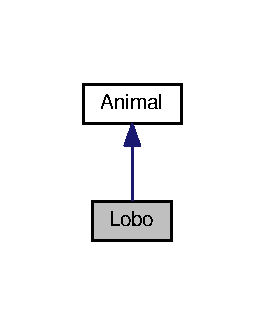
\includegraphics[width=127pt]{classLobo__inherit__graph}
\end{center}
\end{figure}


Collaboration diagram for Lobo\+:
\nopagebreak
\begin{figure}[H]
\begin{center}
\leavevmode
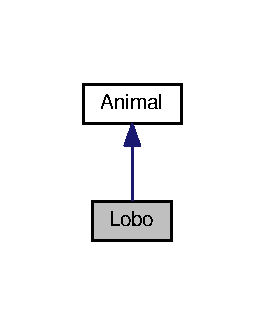
\includegraphics[width=127pt]{classLobo__coll__graph}
\end{center}
\end{figure}
\subsection*{Public Member Functions}
\begin{DoxyCompactItemize}
\item 
\hyperlink{classLobo_a5c6b593887d794ea47abcc7af82a4090}{Lobo} ()
\begin{DoxyCompactList}\small\item\em Constructor por defecto. \end{DoxyCompactList}\item 
\hyperlink{classLobo_a2424bb5ebc7f52b2255b53c8d1560413}{Lobo} (int \hyperlink{classAnimal_ab403adfd13b57143eff123bdd6a2febb}{Fila}, int \hyperlink{classAnimal_a340d64e6e4ffe5f35e0855c63aad1bd3}{Columna}, int \hyperlink{classAnimal_a42b629ae5a7e0c05263a3f6e592ea116}{Sexo})
\begin{DoxyCompactList}\small\item\em Constructor para crear un \hyperlink{classLobo}{Lobo} con datos especificos. \end{DoxyCompactList}\item 
virtual \hyperlink{classLobo_ac3f55f7ba044fc5a20fbcbeed644ce54}{$\sim$\+Lobo} ()
\begin{DoxyCompactList}\small\item\em Destructor. \end{DoxyCompactList}\item 
int \hyperlink{classLobo_af373be32ff2bc56162b7886e3de4b8c5}{Mover} (int columns, int rows, \hyperlink{classCelda}{Celda} $\ast$$\ast$$\ast$terreno)
\begin{DoxyCompactList}\small\item\em Metodo para que el \hyperlink{classLobo}{Lobo} se mueva en el terreno. Es capaz de moverse hasta tres espacios en el terrreno siempre que estan desocupados y sean aledaños. \end{DoxyCompactList}\item 
int \hyperlink{classLobo_a6da7977c9f5f955b20919648345ca550}{Comer} (int columns, int rows, \hyperlink{classCelda}{Celda} $\ast$$\ast$$\ast$terreno)
\begin{DoxyCompactList}\small\item\em Metodo para comer. Se alimenta de cualquier otro animal que esten en posiciones aledañas. Recive 10 puntos por Ovejas, 5 puntos por Zorros y 2 por ratones. Mata al otro animal. No puede excederse de 100 la energia del \hyperlink{classZorro}{Zorro}. Si hay dos lobos machos alguno de los dos muere. \end{DoxyCompactList}\item 
void \hyperlink{classLobo_a79ea0886836c5c493a8bac08ef32db5c}{Reproducir} (int columns, int rows, \hyperlink{classCelda}{Celda} $\ast$$\ast$$\ast$terreno)
\begin{DoxyCompactList}\small\item\em Metodo para reproducirse. Solo se puede reproducir con un animal y solo si es de su misma especie pero de distinto sexo si se reproduce tanto este como la pareja no puede volver a resproducirse durante el dia. \end{DoxyCompactList}\end{DoxyCompactItemize}
\subsection*{Additional Inherited Members}


\subsection{Constructor \& Destructor Documentation}
\index{Lobo@{Lobo}!Lobo@{Lobo}}
\index{Lobo@{Lobo}!Lobo@{Lobo}}
\subsubsection[{\texorpdfstring{Lobo()}{Lobo()}}]{\setlength{\rightskip}{0pt plus 5cm}Lobo\+::\+Lobo (
\begin{DoxyParamCaption}
{}
\end{DoxyParamCaption}
)}\hypertarget{classLobo_a5c6b593887d794ea47abcc7af82a4090}{}\label{classLobo_a5c6b593887d794ea47abcc7af82a4090}


Constructor por defecto. 

\index{Lobo@{Lobo}!Lobo@{Lobo}}
\index{Lobo@{Lobo}!Lobo@{Lobo}}
\subsubsection[{\texorpdfstring{Lobo(int Fila, int Columna, int Sexo)}{Lobo(int Fila, int Columna, int Sexo)}}]{\setlength{\rightskip}{0pt plus 5cm}Lobo\+::\+Lobo (
\begin{DoxyParamCaption}
\item[{int}]{Fila, }
\item[{int}]{Columna, }
\item[{int}]{Sexo}
\end{DoxyParamCaption}
)}\hypertarget{classLobo_a2424bb5ebc7f52b2255b53c8d1560413}{}\label{classLobo_a2424bb5ebc7f52b2255b53c8d1560413}


Constructor para crear un \hyperlink{classLobo}{Lobo} con datos especificos. 

\index{Lobo@{Lobo}!````~Lobo@{$\sim$\+Lobo}}
\index{````~Lobo@{$\sim$\+Lobo}!Lobo@{Lobo}}
\subsubsection[{\texorpdfstring{$\sim$\+Lobo()}{~Lobo()}}]{\setlength{\rightskip}{0pt plus 5cm}Lobo\+::$\sim$\+Lobo (
\begin{DoxyParamCaption}
{}
\end{DoxyParamCaption}
)\hspace{0.3cm}{\ttfamily [virtual]}}\hypertarget{classLobo_ac3f55f7ba044fc5a20fbcbeed644ce54}{}\label{classLobo_ac3f55f7ba044fc5a20fbcbeed644ce54}


Destructor. 



\subsection{Member Function Documentation}
\index{Lobo@{Lobo}!Comer@{Comer}}
\index{Comer@{Comer}!Lobo@{Lobo}}
\subsubsection[{\texorpdfstring{Comer(int columns, int rows, Celda $\ast$$\ast$$\ast$terreno)}{Comer(int columns, int rows, Celda ***terreno)}}]{\setlength{\rightskip}{0pt plus 5cm}int Lobo\+::\+Comer (
\begin{DoxyParamCaption}
\item[{int}]{columns, }
\item[{int}]{rows, }
\item[{{\bf Celda} $\ast$$\ast$$\ast$}]{terreno}
\end{DoxyParamCaption}
)\hspace{0.3cm}{\ttfamily [virtual]}}\hypertarget{classLobo_a6da7977c9f5f955b20919648345ca550}{}\label{classLobo_a6da7977c9f5f955b20919648345ca550}


Metodo para comer. Se alimenta de cualquier otro animal que esten en posiciones aledañas. Recive 10 puntos por Ovejas, 5 puntos por Zorros y 2 por ratones. Mata al otro animal. No puede excederse de 100 la energia del \hyperlink{classZorro}{Zorro}. Si hay dos lobos machos alguno de los dos muere. 



Implements \hyperlink{classAnimal_a4ce5ddb28b7784d6ff7293f312fb5d0a}{Animal}.

\index{Lobo@{Lobo}!Mover@{Mover}}
\index{Mover@{Mover}!Lobo@{Lobo}}
\subsubsection[{\texorpdfstring{Mover(int columns, int rows, Celda $\ast$$\ast$$\ast$terreno)}{Mover(int columns, int rows, Celda ***terreno)}}]{\setlength{\rightskip}{0pt plus 5cm}int Lobo\+::\+Mover (
\begin{DoxyParamCaption}
\item[{int}]{columns, }
\item[{int}]{rows, }
\item[{{\bf Celda} $\ast$$\ast$$\ast$}]{terreno}
\end{DoxyParamCaption}
)\hspace{0.3cm}{\ttfamily [virtual]}}\hypertarget{classLobo_af373be32ff2bc56162b7886e3de4b8c5}{}\label{classLobo_af373be32ff2bc56162b7886e3de4b8c5}


Metodo para que el \hyperlink{classLobo}{Lobo} se mueva en el terreno. Es capaz de moverse hasta tres espacios en el terrreno siempre que estan desocupados y sean aledaños. 


\begin{DoxyParams}{Parameters}
{\em x\+Actual} & Posicion actual del animal. \\
\hline
{\em y\+Actual} & Posicion actual del animal. \\
\hline
{\em x\+Previo} & Posicion previa del animal. \\
\hline
{\em y\+Previo} & Posicion previa del animal. \\
\hline
{\em contador} & Numero de veces que se ha desplzado el animal. \\
\hline
\end{DoxyParams}


Implements \hyperlink{classAnimal_acfb4b1ab56fbd8d98b9ddc4070df6521}{Animal}.

\index{Lobo@{Lobo}!Reproducir@{Reproducir}}
\index{Reproducir@{Reproducir}!Lobo@{Lobo}}
\subsubsection[{\texorpdfstring{Reproducir(int columns, int rows, Celda $\ast$$\ast$$\ast$terreno)}{Reproducir(int columns, int rows, Celda ***terreno)}}]{\setlength{\rightskip}{0pt plus 5cm}void Lobo\+::\+Reproducir (
\begin{DoxyParamCaption}
\item[{int}]{columns, }
\item[{int}]{rows, }
\item[{{\bf Celda} $\ast$$\ast$$\ast$}]{terreno}
\end{DoxyParamCaption}
)\hspace{0.3cm}{\ttfamily [virtual]}}\hypertarget{classLobo_a79ea0886836c5c493a8bac08ef32db5c}{}\label{classLobo_a79ea0886836c5c493a8bac08ef32db5c}


Metodo para reproducirse. Solo se puede reproducir con un animal y solo si es de su misma especie pero de distinto sexo si se reproduce tanto este como la pareja no puede volver a resproducirse durante el dia. 


\begin{DoxyParams}{Parameters}
{\em reproduzcase} & Mediante esta variable se informa si hay una pareja disponible. \\
\hline
{\em x} & Posicion del animal con el cual se puede reproducir. \\
\hline
{\em y} & Posicion del animal con el cual se puede reproducir. \\
\hline
\end{DoxyParams}


Implements \hyperlink{classAnimal_aec115272cec5fc59c1a6944a0ad43fef}{Animal}.



The documentation for this class was generated from the following files\+:\begin{DoxyCompactItemize}
\item 
\hyperlink{Lobo_8h}{Lobo.\+h}\item 
\hyperlink{Lobo_8cpp}{Lobo.\+cpp}\end{DoxyCompactItemize}

\hypertarget{classOveja}{}\section{Oveja Class Reference}
\label{classOveja}\index{Oveja@{Oveja}}


{\ttfamily \#include $<$Oveja.\+h$>$}



Inheritance diagram for Oveja\+:
\nopagebreak
\begin{figure}[H]
\begin{center}
\leavevmode
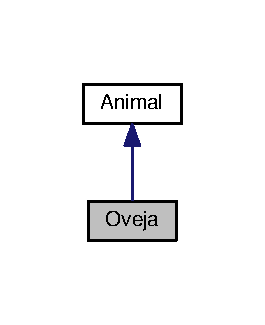
\includegraphics[width=127pt]{classOveja__inherit__graph}
\end{center}
\end{figure}


Collaboration diagram for Oveja\+:
\nopagebreak
\begin{figure}[H]
\begin{center}
\leavevmode
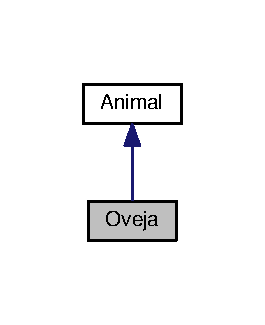
\includegraphics[width=127pt]{classOveja__coll__graph}
\end{center}
\end{figure}
\subsection*{Public Member Functions}
\begin{DoxyCompactItemize}
\item 
\hyperlink{classOveja_a816d51452247a98f55372b7407de0366}{Oveja} ()
\begin{DoxyCompactList}\small\item\em Constructor por defecto. \end{DoxyCompactList}\item 
\hyperlink{classOveja_a28cf77d31dc8d1770f52380a1ba1088e}{Oveja} (int \hyperlink{classAnimal_ab403adfd13b57143eff123bdd6a2febb}{Fila}, int \hyperlink{classAnimal_a340d64e6e4ffe5f35e0855c63aad1bd3}{Columna}, int \hyperlink{classAnimal_a42b629ae5a7e0c05263a3f6e592ea116}{Sexo})
\begin{DoxyCompactList}\small\item\em Constructor para crear una \hyperlink{classOveja}{Oveja} con datos especificos. \end{DoxyCompactList}\item 
virtual \hyperlink{classOveja_a90e76a79dba9138b13c26ba0b1b3c2cf}{$\sim$\+Oveja} ()
\begin{DoxyCompactList}\small\item\em Destructor. \end{DoxyCompactList}\item 
int \hyperlink{classOveja_acd0a8a66853f3b0937b03ccd4d9d4b58}{Mover} (int columns, int rows, \hyperlink{classCelda}{Celda} $\ast$$\ast$$\ast$terreno)
\begin{DoxyCompactList}\small\item\em Metodo para que la oveja se mueva en el terreno. Es capaz de moverse hasta dos espacios en el terrreno siempre que estan desocupados y sean aledaños. \end{DoxyCompactList}\item 
int \hyperlink{classOveja_ac22b74a090e0a74a945ff07530192540}{Comer} (int columns, int rows, \hyperlink{classCelda}{Celda} $\ast$$\ast$$\ast$terreno)
\begin{DoxyCompactList}\small\item\em Metodo para comer. Se alimenta del zacate, consume 10 puntos del zacate y recupera la misma cantidad. En caso de no haber suficiente zacate, consume lo que haya y recupera eso mismo. No puede excederse de 75 la energia de la oveja. \end{DoxyCompactList}\item 
void \hyperlink{classOveja_af97a947a8b74d64e0fac191aad43e2d7}{Reproducir} (int columns, int rows, \hyperlink{classCelda}{Celda} $\ast$$\ast$$\ast$terreno)
\begin{DoxyCompactList}\small\item\em Metodo para reproducirse. Solo se puede reproducir con un animal y solo si es de su misma especie pero de distinto sexo si se reproduce tanto este como la pareja no puede volver a resproducirse durante el dia. \end{DoxyCompactList}\end{DoxyCompactItemize}
\subsection*{Additional Inherited Members}


\subsection{Constructor \& Destructor Documentation}
\index{Oveja@{Oveja}!Oveja@{Oveja}}
\index{Oveja@{Oveja}!Oveja@{Oveja}}
\subsubsection[{\texorpdfstring{Oveja()}{Oveja()}}]{\setlength{\rightskip}{0pt plus 5cm}Oveja\+::\+Oveja (
\begin{DoxyParamCaption}
{}
\end{DoxyParamCaption}
)}\hypertarget{classOveja_a816d51452247a98f55372b7407de0366}{}\label{classOveja_a816d51452247a98f55372b7407de0366}


Constructor por defecto. 

\index{Oveja@{Oveja}!Oveja@{Oveja}}
\index{Oveja@{Oveja}!Oveja@{Oveja}}
\subsubsection[{\texorpdfstring{Oveja(int Fila, int Columna, int Sexo)}{Oveja(int Fila, int Columna, int Sexo)}}]{\setlength{\rightskip}{0pt plus 5cm}Oveja\+::\+Oveja (
\begin{DoxyParamCaption}
\item[{int}]{Fila, }
\item[{int}]{Columna, }
\item[{int}]{Sexo}
\end{DoxyParamCaption}
)}\hypertarget{classOveja_a28cf77d31dc8d1770f52380a1ba1088e}{}\label{classOveja_a28cf77d31dc8d1770f52380a1ba1088e}


Constructor para crear una \hyperlink{classOveja}{Oveja} con datos especificos. 

\index{Oveja@{Oveja}!````~Oveja@{$\sim$\+Oveja}}
\index{````~Oveja@{$\sim$\+Oveja}!Oveja@{Oveja}}
\subsubsection[{\texorpdfstring{$\sim$\+Oveja()}{~Oveja()}}]{\setlength{\rightskip}{0pt plus 5cm}Oveja\+::$\sim$\+Oveja (
\begin{DoxyParamCaption}
{}
\end{DoxyParamCaption}
)\hspace{0.3cm}{\ttfamily [virtual]}}\hypertarget{classOveja_a90e76a79dba9138b13c26ba0b1b3c2cf}{}\label{classOveja_a90e76a79dba9138b13c26ba0b1b3c2cf}


Destructor. 



\subsection{Member Function Documentation}
\index{Oveja@{Oveja}!Comer@{Comer}}
\index{Comer@{Comer}!Oveja@{Oveja}}
\subsubsection[{\texorpdfstring{Comer(int columns, int rows, Celda $\ast$$\ast$$\ast$terreno)}{Comer(int columns, int rows, Celda ***terreno)}}]{\setlength{\rightskip}{0pt plus 5cm}int Oveja\+::\+Comer (
\begin{DoxyParamCaption}
\item[{int}]{columns, }
\item[{int}]{rows, }
\item[{{\bf Celda} $\ast$$\ast$$\ast$}]{terreno}
\end{DoxyParamCaption}
)\hspace{0.3cm}{\ttfamily [virtual]}}\hypertarget{classOveja_ac22b74a090e0a74a945ff07530192540}{}\label{classOveja_ac22b74a090e0a74a945ff07530192540}


Metodo para comer. Se alimenta del zacate, consume 10 puntos del zacate y recupera la misma cantidad. En caso de no haber suficiente zacate, consume lo que haya y recupera eso mismo. No puede excederse de 75 la energia de la oveja. 



Implements \hyperlink{classAnimal_a4ce5ddb28b7784d6ff7293f312fb5d0a}{Animal}.

\index{Oveja@{Oveja}!Mover@{Mover}}
\index{Mover@{Mover}!Oveja@{Oveja}}
\subsubsection[{\texorpdfstring{Mover(int columns, int rows, Celda $\ast$$\ast$$\ast$terreno)}{Mover(int columns, int rows, Celda ***terreno)}}]{\setlength{\rightskip}{0pt plus 5cm}int Oveja\+::\+Mover (
\begin{DoxyParamCaption}
\item[{int}]{columns, }
\item[{int}]{rows, }
\item[{{\bf Celda} $\ast$$\ast$$\ast$}]{terreno}
\end{DoxyParamCaption}
)\hspace{0.3cm}{\ttfamily [virtual]}}\hypertarget{classOveja_acd0a8a66853f3b0937b03ccd4d9d4b58}{}\label{classOveja_acd0a8a66853f3b0937b03ccd4d9d4b58}


Metodo para que la oveja se mueva en el terreno. Es capaz de moverse hasta dos espacios en el terrreno siempre que estan desocupados y sean aledaños. 


\begin{DoxyParams}{Parameters}
{\em x\+Actual} & Posicion actual del animal. \\
\hline
{\em y\+Actual} & Posicion actual del animal. \\
\hline
{\em x\+Previo} & Posicion previa del animal. \\
\hline
{\em y\+Previo} & Posicion previa del animal. \\
\hline
{\em contador} & Numero de veces que se ha desplzado el animal. \\
\hline
\end{DoxyParams}


Implements \hyperlink{classAnimal_acfb4b1ab56fbd8d98b9ddc4070df6521}{Animal}.

\index{Oveja@{Oveja}!Reproducir@{Reproducir}}
\index{Reproducir@{Reproducir}!Oveja@{Oveja}}
\subsubsection[{\texorpdfstring{Reproducir(int columns, int rows, Celda $\ast$$\ast$$\ast$terreno)}{Reproducir(int columns, int rows, Celda ***terreno)}}]{\setlength{\rightskip}{0pt plus 5cm}void Oveja\+::\+Reproducir (
\begin{DoxyParamCaption}
\item[{int}]{columns, }
\item[{int}]{rows, }
\item[{{\bf Celda} $\ast$$\ast$$\ast$}]{terreno}
\end{DoxyParamCaption}
)\hspace{0.3cm}{\ttfamily [virtual]}}\hypertarget{classOveja_af97a947a8b74d64e0fac191aad43e2d7}{}\label{classOveja_af97a947a8b74d64e0fac191aad43e2d7}


Metodo para reproducirse. Solo se puede reproducir con un animal y solo si es de su misma especie pero de distinto sexo si se reproduce tanto este como la pareja no puede volver a resproducirse durante el dia. 


\begin{DoxyParams}{Parameters}
{\em reproduzcase} & Mediante esta variable se informa si hay una pareja disponible. \\
\hline
{\em x} & Posicion del animal con el cual se puede reproducir. \\
\hline
{\em y} & Posicion del animal con el cual se puede reproducir. \\
\hline
\end{DoxyParams}


Implements \hyperlink{classAnimal_aec115272cec5fc59c1a6944a0ad43fef}{Animal}.



The documentation for this class was generated from the following files\+:\begin{DoxyCompactItemize}
\item 
\hyperlink{Oveja_8h}{Oveja.\+h}\item 
\hyperlink{Oveja_8cpp}{Oveja.\+cpp}\end{DoxyCompactItemize}

\hypertarget{classRaton}{}\section{Raton Class Reference}
\label{classRaton}\index{Raton@{Raton}}


{\ttfamily \#include $<$Raton.\+h$>$}



Inheritance diagram for Raton\+:\nopagebreak
\begin{figure}[H]
\begin{center}
\leavevmode
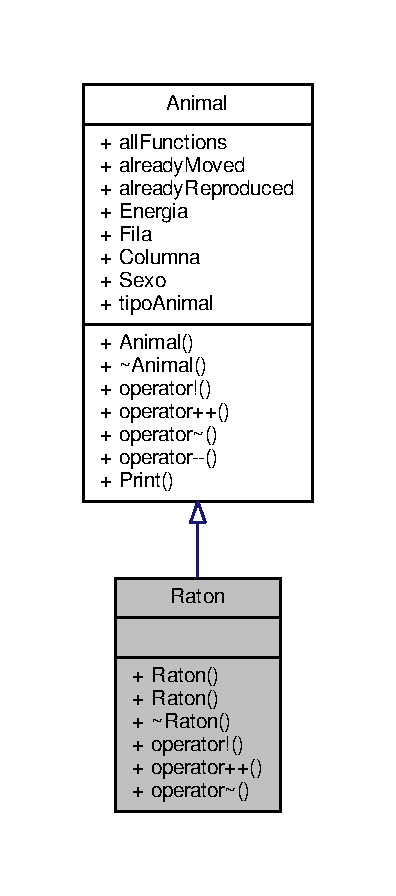
\includegraphics[width=190pt]{classRaton__inherit__graph}
\end{center}
\end{figure}


Collaboration diagram for Raton\+:\nopagebreak
\begin{figure}[H]
\begin{center}
\leavevmode
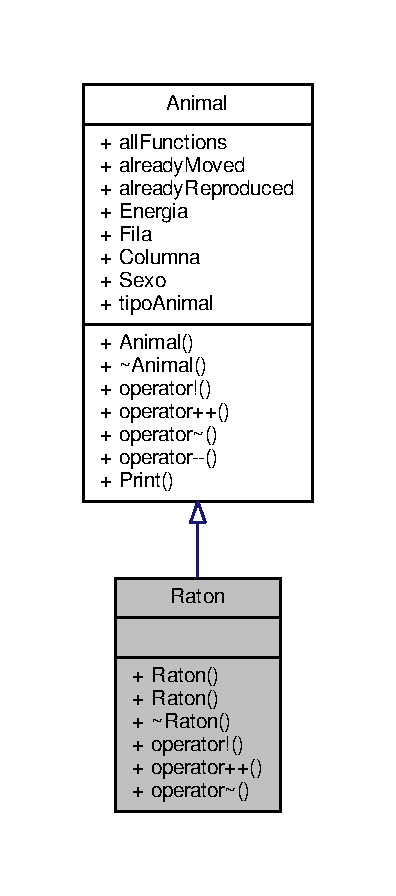
\includegraphics[width=190pt]{classRaton__coll__graph}
\end{center}
\end{figure}
\subsection*{Public Member Functions}
\begin{DoxyCompactItemize}
\item 
\hyperlink{classRaton_a9981955d139254e7a3990ebbf4d6d6d2}{Raton} ()
\begin{DoxyCompactList}\small\item\em Constructor por defecto. \end{DoxyCompactList}\item 
\hyperlink{classRaton_abd3b46771d6db783f207274aab538783}{Raton} (int \hyperlink{classAnimal_ab403adfd13b57143eff123bdd6a2febb}{Fila}, int \hyperlink{classAnimal_a340d64e6e4ffe5f35e0855c63aad1bd3}{Columna}, int \hyperlink{classAnimal_a42b629ae5a7e0c05263a3f6e592ea116}{Sexo})
\begin{DoxyCompactList}\small\item\em Constructor para crear un \hyperlink{classRaton}{Raton} con datos especificos. \end{DoxyCompactList}\item 
virtual \hyperlink{classRaton_a65e9e02f328adbda8d588548a3b1d76b}{$\sim$\+Raton} ()
\begin{DoxyCompactList}\small\item\em Destructor. \end{DoxyCompactList}\item 
int \hyperlink{classRaton_ad50cebe48f49dbadef570d616a0e6aa3}{operator!} ()
\begin{DoxyCompactList}\small\item\em Metodo para que el raton se mueva en el terreno. Es capaz de moverse solo un espacio en el terrreno siempre que este desocupado y sea aledaño. \end{DoxyCompactList}\item 
int \hyperlink{classRaton_a64ec37f911376e16802ad5906bb4e27a}{operator++} ()
\begin{DoxyCompactList}\small\item\em Metodo para comer. Se alimenta del zacate, consume 5 puntos del zacate y recupera la misma cantidad. En caso de no haber suficiente zacate, consume lo que haya y recupera eso mismo. No puede excederse de 25 la energia del \hyperlink{classRaton}{Raton}. \end{DoxyCompactList}\item 
void \hyperlink{classRaton_a7ec71ea95a98d13bf2cccf108b3c76d6}{operator$\sim$} ()
\begin{DoxyCompactList}\small\item\em Metodo para reproducirse. Solo se puede reproducir con un animal y solo si es de su misma especie pero de distinto sexo si se reproduce tanto este como la pareja no puede volver a resproducirse durante el dia. \end{DoxyCompactList}\end{DoxyCompactItemize}
\subsection*{Additional Inherited Members}


\subsection{Constructor \& Destructor Documentation}
\index{Raton@{Raton}!Raton@{Raton}}
\index{Raton@{Raton}!Raton@{Raton}}
\subsubsection[{\texorpdfstring{Raton()}{Raton()}}]{\setlength{\rightskip}{0pt plus 5cm}Raton\+::\+Raton (
\begin{DoxyParamCaption}
{}
\end{DoxyParamCaption}
)}\hypertarget{classRaton_a9981955d139254e7a3990ebbf4d6d6d2}{}\label{classRaton_a9981955d139254e7a3990ebbf4d6d6d2}


Constructor por defecto. 

\index{Raton@{Raton}!Raton@{Raton}}
\index{Raton@{Raton}!Raton@{Raton}}
\subsubsection[{\texorpdfstring{Raton(int Fila, int Columna, int Sexo)}{Raton(int Fila, int Columna, int Sexo)}}]{\setlength{\rightskip}{0pt plus 5cm}Raton\+::\+Raton (
\begin{DoxyParamCaption}
\item[{int}]{Fila, }
\item[{int}]{Columna, }
\item[{int}]{Sexo}
\end{DoxyParamCaption}
)}\hypertarget{classRaton_abd3b46771d6db783f207274aab538783}{}\label{classRaton_abd3b46771d6db783f207274aab538783}


Constructor para crear un \hyperlink{classRaton}{Raton} con datos especificos. 

\index{Raton@{Raton}!````~Raton@{$\sim$\+Raton}}
\index{````~Raton@{$\sim$\+Raton}!Raton@{Raton}}
\subsubsection[{\texorpdfstring{$\sim$\+Raton()}{~Raton()}}]{\setlength{\rightskip}{0pt plus 5cm}Raton\+::$\sim$\+Raton (
\begin{DoxyParamCaption}
{}
\end{DoxyParamCaption}
)\hspace{0.3cm}{\ttfamily [virtual]}}\hypertarget{classRaton_a65e9e02f328adbda8d588548a3b1d76b}{}\label{classRaton_a65e9e02f328adbda8d588548a3b1d76b}


Destructor. 



\subsection{Member Function Documentation}
\index{Raton@{Raton}!operator"!@{operator"!}}
\index{operator"!@{operator"!}!Raton@{Raton}}
\subsubsection[{\texorpdfstring{operator"!()}{operator!()}}]{\setlength{\rightskip}{0pt plus 5cm}int Raton\+::operator! (
\begin{DoxyParamCaption}
{}
\end{DoxyParamCaption}
)\hspace{0.3cm}{\ttfamily [virtual]}}\hypertarget{classRaton_ad50cebe48f49dbadef570d616a0e6aa3}{}\label{classRaton_ad50cebe48f49dbadef570d616a0e6aa3}


Metodo para que el raton se mueva en el terreno. Es capaz de moverse solo un espacio en el terrreno siempre que este desocupado y sea aledaño. 



Implements \hyperlink{classAnimal_abe502d1333df77d245d74cd20190a0aa}{Animal}.

\index{Raton@{Raton}!operator++@{operator++}}
\index{operator++@{operator++}!Raton@{Raton}}
\subsubsection[{\texorpdfstring{operator++()}{operator++()}}]{\setlength{\rightskip}{0pt plus 5cm}int Raton\+::operator++ (
\begin{DoxyParamCaption}
{}
\end{DoxyParamCaption}
)\hspace{0.3cm}{\ttfamily [virtual]}}\hypertarget{classRaton_a64ec37f911376e16802ad5906bb4e27a}{}\label{classRaton_a64ec37f911376e16802ad5906bb4e27a}


Metodo para comer. Se alimenta del zacate, consume 5 puntos del zacate y recupera la misma cantidad. En caso de no haber suficiente zacate, consume lo que haya y recupera eso mismo. No puede excederse de 25 la energia del \hyperlink{classRaton}{Raton}. 



Implements \hyperlink{classAnimal_a66e3bc83959ea5c5d7aa8d85f8ca993c}{Animal}.

\index{Raton@{Raton}!operator````~@{operator$\sim$}}
\index{operator````~@{operator$\sim$}!Raton@{Raton}}
\subsubsection[{\texorpdfstring{operator$\sim$()}{operator~()}}]{\setlength{\rightskip}{0pt plus 5cm}void Raton\+::operator$\sim$ (
\begin{DoxyParamCaption}
{}
\end{DoxyParamCaption}
)\hspace{0.3cm}{\ttfamily [virtual]}}\hypertarget{classRaton_a7ec71ea95a98d13bf2cccf108b3c76d6}{}\label{classRaton_a7ec71ea95a98d13bf2cccf108b3c76d6}


Metodo para reproducirse. Solo se puede reproducir con un animal y solo si es de su misma especie pero de distinto sexo si se reproduce tanto este como la pareja no puede volver a resproducirse durante el dia. 


\begin{DoxyParams}{Parameters}
{\em reproduzcase} & Mediante esta variable se informa si hay una pareja disponible. \\
\hline
{\em x} & Posicion del animal con el cual se puede reproducir. \\
\hline
{\em y} & Posicion del animal con el cual se puede reproducir. \\
\hline
\end{DoxyParams}


Implements \hyperlink{classAnimal_a6539ec18d8975982b65de76d8e5638f0}{Animal}.



The documentation for this class was generated from the following files\+:\begin{DoxyCompactItemize}
\item 
\hyperlink{Raton_8h}{Raton.\+h}\item 
\hyperlink{Raton_8cpp}{Raton.\+cpp}\end{DoxyCompactItemize}

\hypertarget{classZorro}{}\section{Zorro Class Reference}
\label{classZorro}\index{Zorro@{Zorro}}


{\ttfamily \#include $<$Zorro.\+h$>$}



Inheritance diagram for Zorro\+:
\nopagebreak
\begin{figure}[H]
\begin{center}
\leavevmode
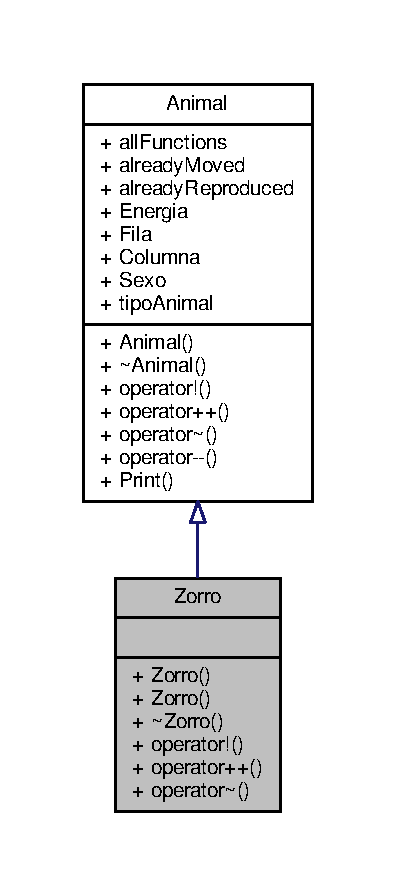
\includegraphics[width=127pt]{classZorro__inherit__graph}
\end{center}
\end{figure}


Collaboration diagram for Zorro\+:
\nopagebreak
\begin{figure}[H]
\begin{center}
\leavevmode
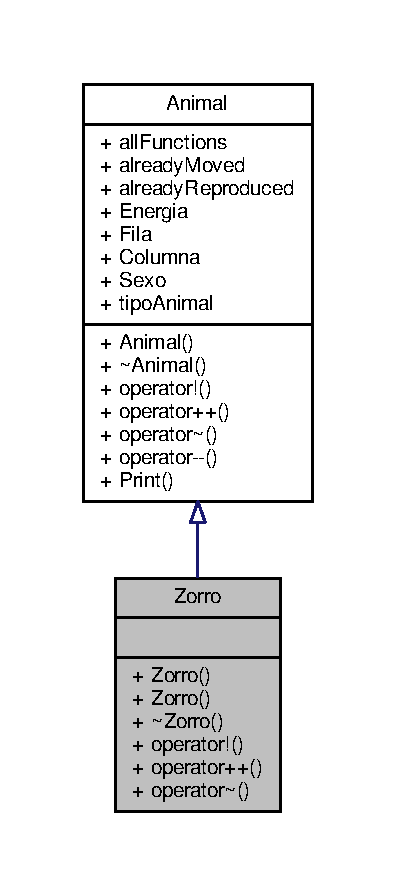
\includegraphics[width=127pt]{classZorro__coll__graph}
\end{center}
\end{figure}
\subsection*{Public Member Functions}
\begin{DoxyCompactItemize}
\item 
\hyperlink{classZorro_adb6072a36faa243b1c185ec3e566f556}{Zorro} ()
\begin{DoxyCompactList}\small\item\em Constructor por defecto. \end{DoxyCompactList}\item 
\hyperlink{classZorro_a16f7f378084d2fa795750d1ff824ca76}{Zorro} (int \hyperlink{classAnimal_ab403adfd13b57143eff123bdd6a2febb}{Fila}, int \hyperlink{classAnimal_a340d64e6e4ffe5f35e0855c63aad1bd3}{Columna}, int \hyperlink{classAnimal_a42b629ae5a7e0c05263a3f6e592ea116}{Sexo})
\begin{DoxyCompactList}\small\item\em Constructor para crear un \hyperlink{classZorro}{Zorro} con datos especificos. \end{DoxyCompactList}\item 
virtual \hyperlink{classZorro_a73fe75fd4746a9347da559ffaa741842}{$\sim$\+Zorro} ()
\begin{DoxyCompactList}\small\item\em Destructor. \end{DoxyCompactList}\item 
int \hyperlink{classZorro_a2facc3ce009fc8d46ff7cbd93370c06b}{Mover} (int columns, int rows, \hyperlink{classCelda}{Celda} $\ast$$\ast$$\ast$terreno)
\begin{DoxyCompactList}\small\item\em Metodo para que el zorro se mueva en el terreno. Es capaz de moverse solo un espacio en el terrreno siempre que este desocupado y sea aledaño. \end{DoxyCompactList}\item 
int \hyperlink{classZorro_aff938c6cbfac969d13261481b6cb4976}{Comer} (int columns, int rows, \hyperlink{classCelda}{Celda} $\ast$$\ast$$\ast$terreno)
\begin{DoxyCompactList}\small\item\em Metodo para Comer. Se alimenta de Ratones que esten en posiciones aledañas, consume 2 puntos y mata al otro animal. No puede excederse de 50 la energia del \hyperlink{classZorro}{Zorro}. \end{DoxyCompactList}\item 
void \hyperlink{classZorro_a22664badacda98773684a81b0c6c29a0}{Reproducir} (int columns, int rows, \hyperlink{classCelda}{Celda} $\ast$$\ast$$\ast$terreno)
\begin{DoxyCompactList}\small\item\em Metodo para reproducirse. Solo se puede reproducir con un animal y solo si es de su misma especie pero de distinto sexo si se reproduce tanto este como la pareja no puede volver a resproducirse durante el dia. \end{DoxyCompactList}\end{DoxyCompactItemize}
\subsection*{Additional Inherited Members}


\subsection{Constructor \& Destructor Documentation}
\index{Zorro@{Zorro}!Zorro@{Zorro}}
\index{Zorro@{Zorro}!Zorro@{Zorro}}
\subsubsection[{\texorpdfstring{Zorro()}{Zorro()}}]{\setlength{\rightskip}{0pt plus 5cm}Zorro\+::\+Zorro (
\begin{DoxyParamCaption}
{}
\end{DoxyParamCaption}
)}\hypertarget{classZorro_adb6072a36faa243b1c185ec3e566f556}{}\label{classZorro_adb6072a36faa243b1c185ec3e566f556}


Constructor por defecto. 

\index{Zorro@{Zorro}!Zorro@{Zorro}}
\index{Zorro@{Zorro}!Zorro@{Zorro}}
\subsubsection[{\texorpdfstring{Zorro(int Fila, int Columna, int Sexo)}{Zorro(int Fila, int Columna, int Sexo)}}]{\setlength{\rightskip}{0pt plus 5cm}Zorro\+::\+Zorro (
\begin{DoxyParamCaption}
\item[{int}]{Fila, }
\item[{int}]{Columna, }
\item[{int}]{Sexo}
\end{DoxyParamCaption}
)}\hypertarget{classZorro_a16f7f378084d2fa795750d1ff824ca76}{}\label{classZorro_a16f7f378084d2fa795750d1ff824ca76}


Constructor para crear un \hyperlink{classZorro}{Zorro} con datos especificos. 

\index{Zorro@{Zorro}!````~Zorro@{$\sim$\+Zorro}}
\index{````~Zorro@{$\sim$\+Zorro}!Zorro@{Zorro}}
\subsubsection[{\texorpdfstring{$\sim$\+Zorro()}{~Zorro()}}]{\setlength{\rightskip}{0pt plus 5cm}Zorro\+::$\sim$\+Zorro (
\begin{DoxyParamCaption}
{}
\end{DoxyParamCaption}
)\hspace{0.3cm}{\ttfamily [virtual]}}\hypertarget{classZorro_a73fe75fd4746a9347da559ffaa741842}{}\label{classZorro_a73fe75fd4746a9347da559ffaa741842}


Destructor. 



\subsection{Member Function Documentation}
\index{Zorro@{Zorro}!Comer@{Comer}}
\index{Comer@{Comer}!Zorro@{Zorro}}
\subsubsection[{\texorpdfstring{Comer(int columns, int rows, Celda $\ast$$\ast$$\ast$terreno)}{Comer(int columns, int rows, Celda ***terreno)}}]{\setlength{\rightskip}{0pt plus 5cm}int Zorro\+::\+Comer (
\begin{DoxyParamCaption}
\item[{int}]{columns, }
\item[{int}]{rows, }
\item[{{\bf Celda} $\ast$$\ast$$\ast$}]{terreno}
\end{DoxyParamCaption}
)\hspace{0.3cm}{\ttfamily [virtual]}}\hypertarget{classZorro_aff938c6cbfac969d13261481b6cb4976}{}\label{classZorro_aff938c6cbfac969d13261481b6cb4976}


Metodo para Comer. Se alimenta de Ratones que esten en posiciones aledañas, consume 2 puntos y mata al otro animal. No puede excederse de 50 la energia del \hyperlink{classZorro}{Zorro}. 



Implements \hyperlink{classAnimal_a4ce5ddb28b7784d6ff7293f312fb5d0a}{Animal}.

\index{Zorro@{Zorro}!Mover@{Mover}}
\index{Mover@{Mover}!Zorro@{Zorro}}
\subsubsection[{\texorpdfstring{Mover(int columns, int rows, Celda $\ast$$\ast$$\ast$terreno)}{Mover(int columns, int rows, Celda ***terreno)}}]{\setlength{\rightskip}{0pt plus 5cm}int Zorro\+::\+Mover (
\begin{DoxyParamCaption}
\item[{int}]{columns, }
\item[{int}]{rows, }
\item[{{\bf Celda} $\ast$$\ast$$\ast$}]{terreno}
\end{DoxyParamCaption}
)\hspace{0.3cm}{\ttfamily [virtual]}}\hypertarget{classZorro_a2facc3ce009fc8d46ff7cbd93370c06b}{}\label{classZorro_a2facc3ce009fc8d46ff7cbd93370c06b}


Metodo para que el zorro se mueva en el terreno. Es capaz de moverse solo un espacio en el terrreno siempre que este desocupado y sea aledaño. 


\begin{DoxyParams}{Parameters}
{\em x\+Actual} & Posicion actual del animal. \\
\hline
{\em y\+Actual} & Posicion actual del animal. \\
\hline
{\em x\+Previo} & Posicion previa del animal. \\
\hline
{\em y\+Previo} & Posicion previa del animal. \\
\hline
{\em contador} & Numero de veces que se ha desplzado el animal. \\
\hline
\end{DoxyParams}


Implements \hyperlink{classAnimal_acfb4b1ab56fbd8d98b9ddc4070df6521}{Animal}.

\index{Zorro@{Zorro}!Reproducir@{Reproducir}}
\index{Reproducir@{Reproducir}!Zorro@{Zorro}}
\subsubsection[{\texorpdfstring{Reproducir(int columns, int rows, Celda $\ast$$\ast$$\ast$terreno)}{Reproducir(int columns, int rows, Celda ***terreno)}}]{\setlength{\rightskip}{0pt plus 5cm}void Zorro\+::\+Reproducir (
\begin{DoxyParamCaption}
\item[{int}]{columns, }
\item[{int}]{rows, }
\item[{{\bf Celda} $\ast$$\ast$$\ast$}]{terreno}
\end{DoxyParamCaption}
)\hspace{0.3cm}{\ttfamily [virtual]}}\hypertarget{classZorro_a22664badacda98773684a81b0c6c29a0}{}\label{classZorro_a22664badacda98773684a81b0c6c29a0}


Metodo para reproducirse. Solo se puede reproducir con un animal y solo si es de su misma especie pero de distinto sexo si se reproduce tanto este como la pareja no puede volver a resproducirse durante el dia. 


\begin{DoxyParams}{Parameters}
{\em reproduzcase} & Mediante esta variable se informa si hay una pareja disponible. \\
\hline
{\em x} & Posicion del animal con el cual se puede reproducir. \\
\hline
{\em y} & Posicion del animal con el cual se puede reproducir. \\
\hline
\end{DoxyParams}


Implements \hyperlink{classAnimal_aec115272cec5fc59c1a6944a0ad43fef}{Animal}.



The documentation for this class was generated from the following files\+:\begin{DoxyCompactItemize}
\item 
\hyperlink{Zorro_8h}{Zorro.\+h}\item 
\hyperlink{Zorro_8cpp}{Zorro.\+cpp}\end{DoxyCompactItemize}

\chapter{File Documentation}
\hypertarget{Animal_8cpp}{}\section{Animal.\+cpp File Reference}
\label{Animal_8cpp}\index{Animal.\+cpp@{Animal.\+cpp}}


Clase \hyperlink{classAnimal}{Animal}.  


{\ttfamily \#include \char`\"{}Animal.\+h\char`\"{}}\\*
{\ttfamily \#include \char`\"{}Celda.\+h\char`\"{}}\\*
Include dependency graph for Animal.\+cpp\+:\nopagebreak
\begin{figure}[H]
\begin{center}
\leavevmode
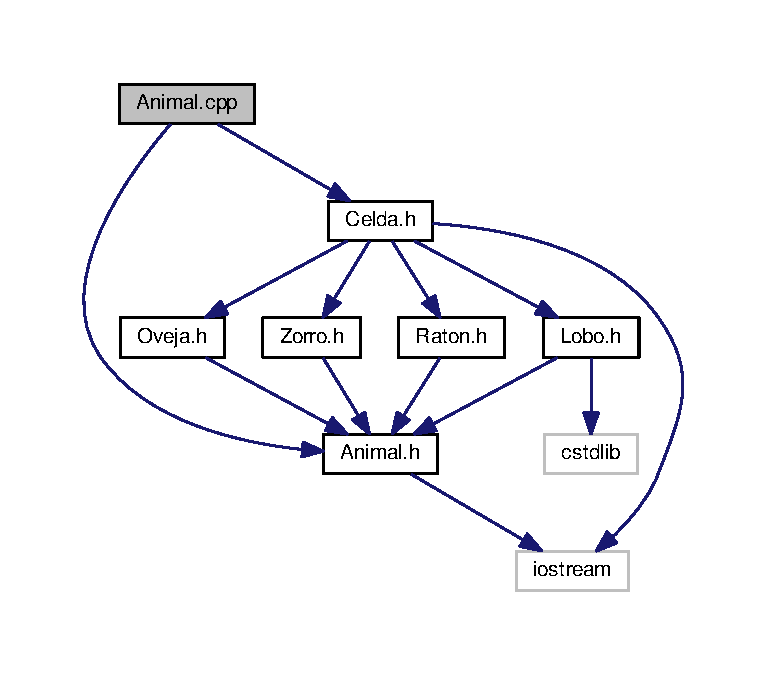
\includegraphics[width=350pt]{Animal_8cpp__incl}
\end{center}
\end{figure}


\subsection{Detailed Description}
Clase \hyperlink{classAnimal}{Animal}. 

\begin{DoxyVersion}{Version}
1.\+0 
\end{DoxyVersion}
\begin{DoxyDate}{Date}
29/01/17 
\end{DoxyDate}
\begin{DoxyAuthor}{Author}
Luis Diego Fernandez, Daniel Jimenez  Juego de la vida 
\end{DoxyAuthor}

\hypertarget{Animal_8h}{}\section{Animal.\+h File Reference}
\label{Animal_8h}\index{Animal.\+h@{Animal.\+h}}
{\ttfamily \#include $<$iostream$>$}\\*
Include dependency graph for Animal.\+h\+:\nopagebreak
\begin{figure}[H]
\begin{center}
\leavevmode
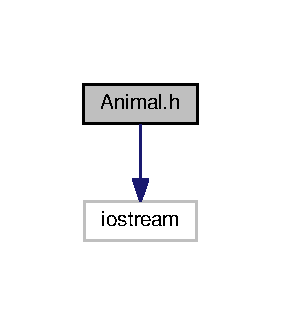
\includegraphics[width=135pt]{Animal_8h__incl}
\end{center}
\end{figure}
This graph shows which files directly or indirectly include this file\+:\nopagebreak
\begin{figure}[H]
\begin{center}
\leavevmode
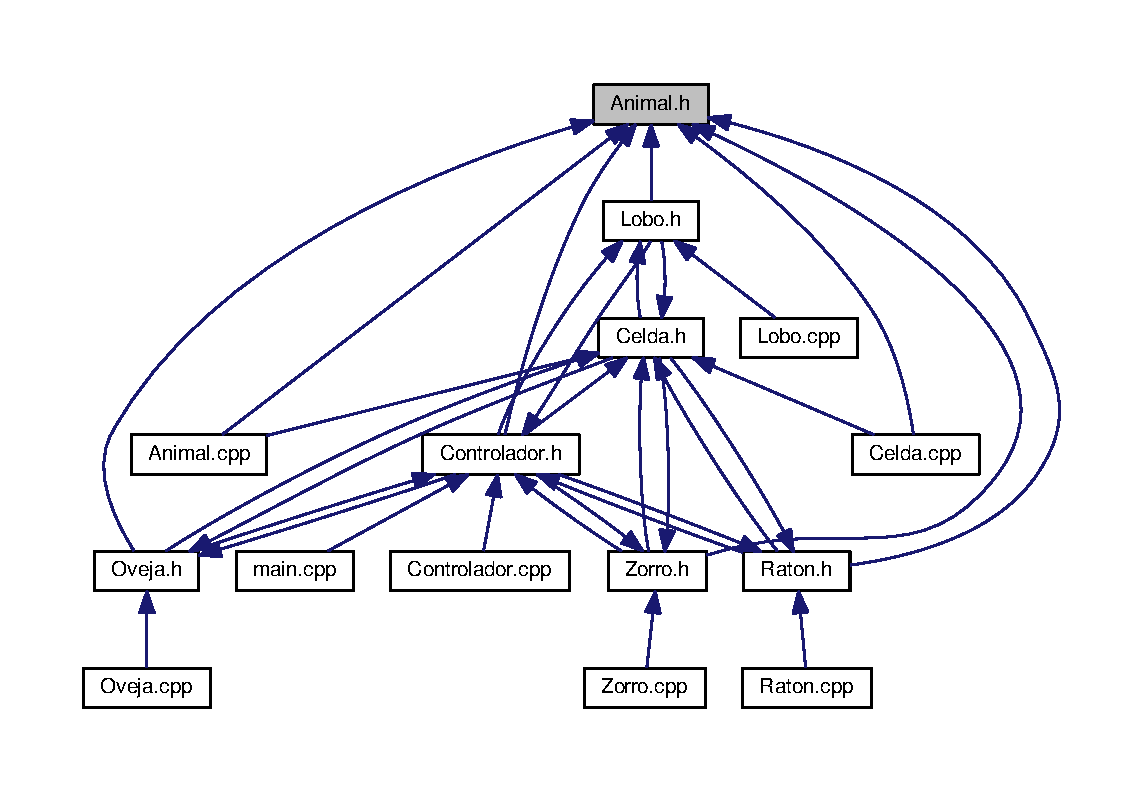
\includegraphics[width=350pt]{Animal_8h__dep__incl}
\end{center}
\end{figure}
\subsection*{Classes}
\begin{DoxyCompactItemize}
\item 
class \hyperlink{classAnimal}{Animal}
\end{DoxyCompactItemize}

\hypertarget{apuntes_8txt}{}\section{apuntes.\+txt File Reference}
\label{apuntes_8txt}\index{apuntes.\+txt@{apuntes.\+txt}}
\subsection*{Variables}
\begin{DoxyCompactItemize}
\item 
El zacate es una variable tipo int Su rango va de\mbox{[}0, 100\mbox{]} Los animales no se van a representar con \hyperlink{apuntes_8txt_a7fafe4330e5347d2a816fe8b3500cb0e}{strings}
\end{DoxyCompactItemize}


\subsection{Variable Documentation}
\index{apuntes.\+txt@{apuntes.\+txt}!strings@{strings}}
\index{strings@{strings}!apuntes.\+txt@{apuntes.\+txt}}
\subsubsection[{\texorpdfstring{strings}{strings}}]{\setlength{\rightskip}{0pt plus 5cm}El zacate es una variable tipo int Su rango va de \mbox{[}0, 100\mbox{]} Los animales no se van a representar con strings}\hypertarget{apuntes_8txt_a7fafe4330e5347d2a816fe8b3500cb0e}{}\label{apuntes_8txt_a7fafe4330e5347d2a816fe8b3500cb0e}

\hypertarget{Celda_8cpp}{}\section{Celda.\+cpp File Reference}
\label{Celda_8cpp}\index{Celda.\+cpp@{Celda.\+cpp}}


Clase \hyperlink{classCelda}{Celda}.  


{\ttfamily \#include \char`\"{}Celda.\+h\char`\"{}}\\*
{\ttfamily \#include \char`\"{}Animal.\+h\char`\"{}}\\*
Include dependency graph for Celda.\+cpp\+:\nopagebreak
\begin{figure}[H]
\begin{center}
\leavevmode
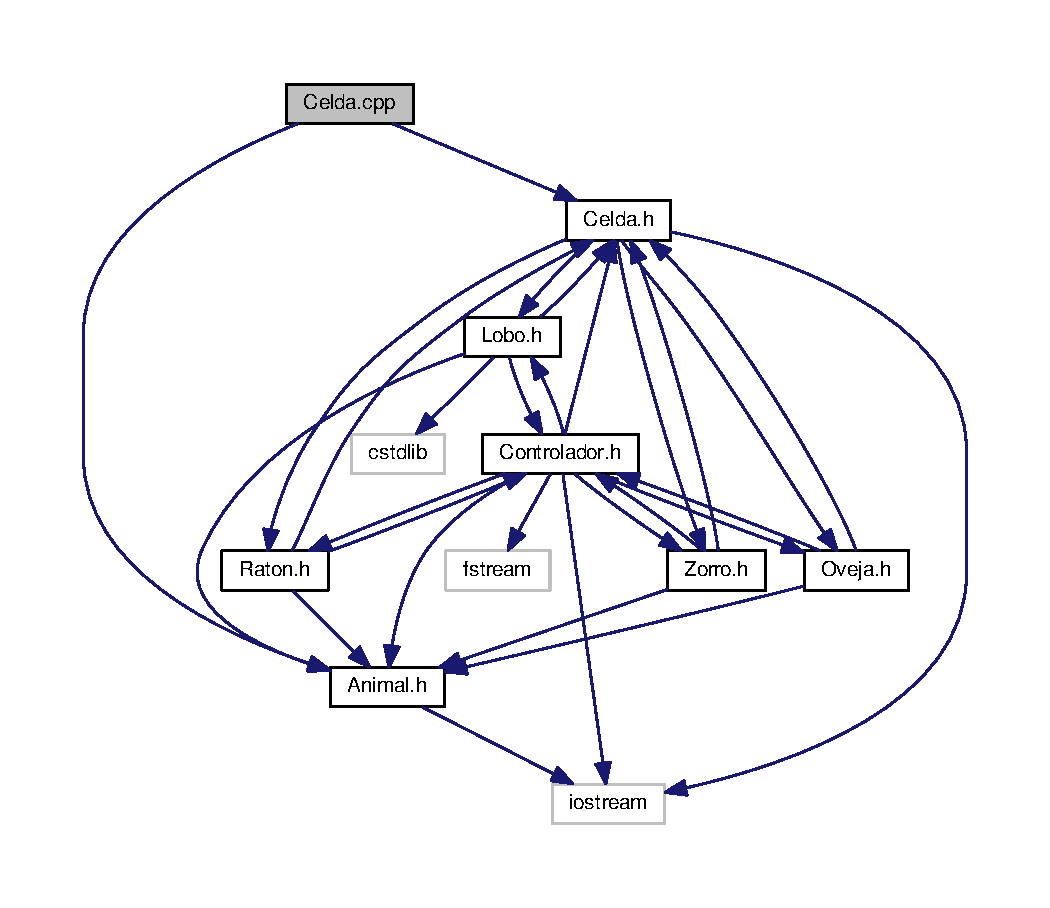
\includegraphics[width=350pt]{Celda_8cpp__incl}
\end{center}
\end{figure}


\subsection{Detailed Description}
Clase \hyperlink{classCelda}{Celda}. 

\begin{DoxyVersion}{Version}
1.\+0 
\end{DoxyVersion}
\begin{DoxyDate}{Date}
29/01/17 
\end{DoxyDate}
\begin{DoxyAuthor}{Author}
Luis Diego Fernandez, Daniel Jimenez  Juego de la vida 
\end{DoxyAuthor}

\hypertarget{Celda_8h}{}\section{Celda.\+h File Reference}
\label{Celda_8h}\index{Celda.\+h@{Celda.\+h}}
{\ttfamily \#include $<$iostream$>$}\\*
{\ttfamily \#include \char`\"{}Lobo.\+h\char`\"{}}\\*
{\ttfamily \#include \char`\"{}Oveja.\+h\char`\"{}}\\*
{\ttfamily \#include \char`\"{}Zorro.\+h\char`\"{}}\\*
{\ttfamily \#include \char`\"{}Raton.\+h\char`\"{}}\\*
Include dependency graph for Celda.\+h\+:
\nopagebreak
\begin{figure}[H]
\begin{center}
\leavevmode
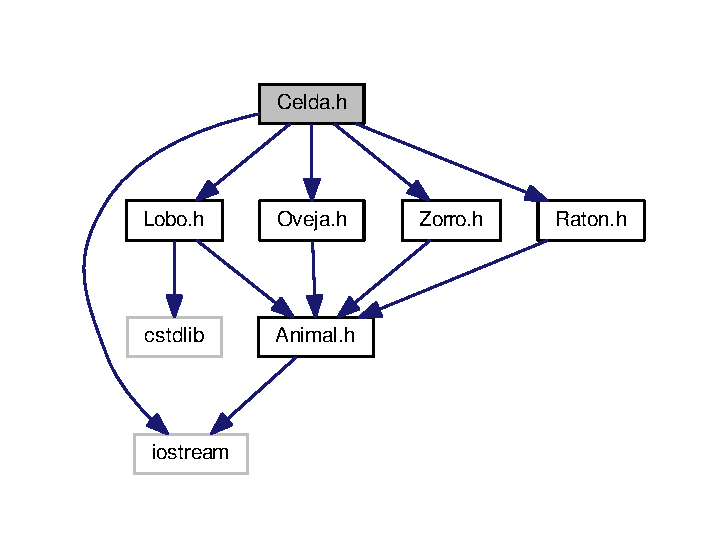
\includegraphics[width=349pt]{Celda_8h__incl}
\end{center}
\end{figure}
This graph shows which files directly or indirectly include this file\+:
\nopagebreak
\begin{figure}[H]
\begin{center}
\leavevmode
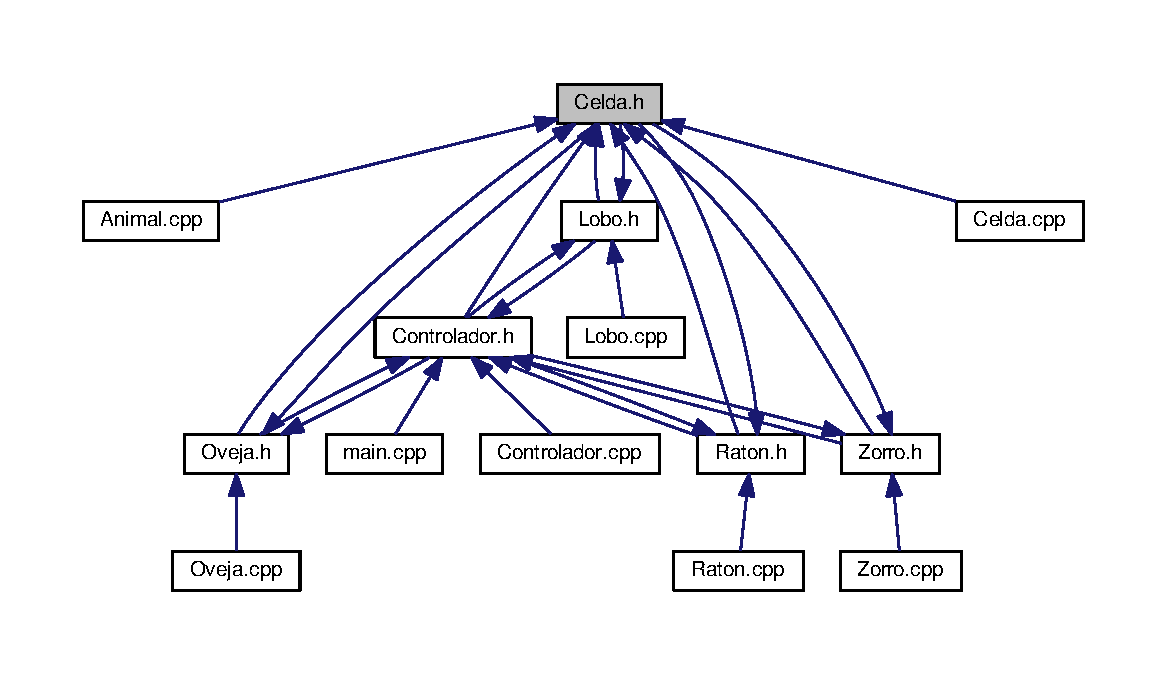
\includegraphics[width=350pt]{Celda_8h__dep__incl}
\end{center}
\end{figure}
\subsection*{Data Structures}
\begin{DoxyCompactItemize}
\item 
class \hyperlink{classCelda}{Celda}
\end{DoxyCompactItemize}

\hypertarget{Controlador_8cpp}{}\section{Controlador.\+cpp File Reference}
\label{Controlador_8cpp}\index{Controlador.\+cpp@{Controlador.\+cpp}}


Clase \hyperlink{classControlador}{Controlador}.  


{\ttfamily \#include \char`\"{}Controlador.\+h\char`\"{}}\\*
Include dependency graph for Controlador.\+cpp\+:
\nopagebreak
\begin{figure}[H]
\begin{center}
\leavevmode
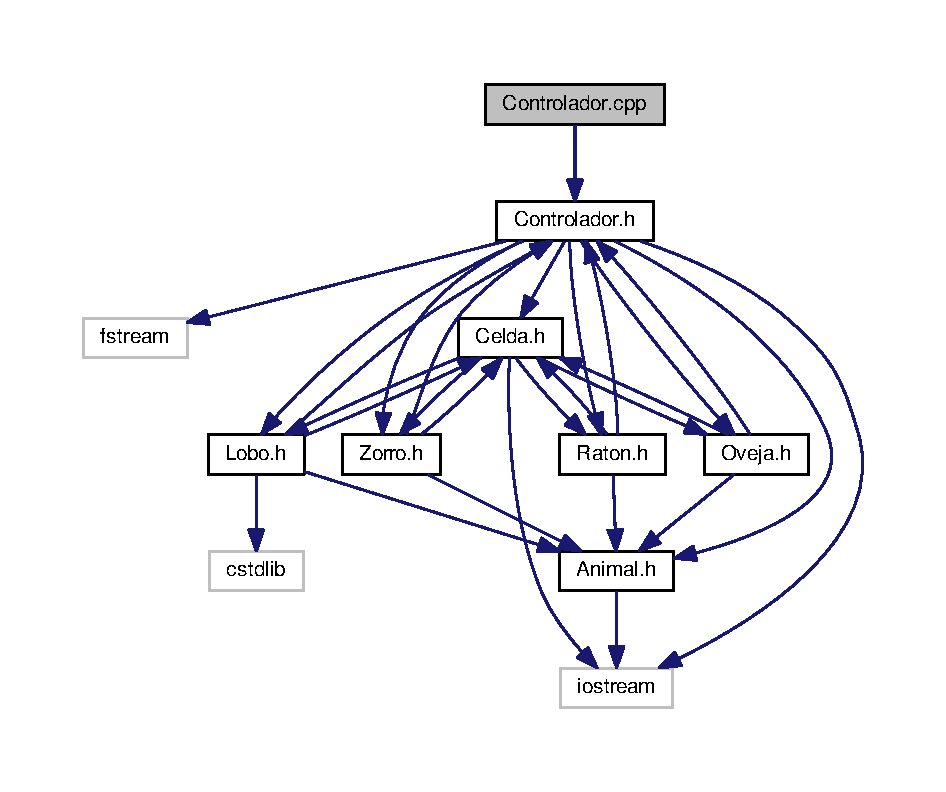
\includegraphics[width=350pt]{Controlador_8cpp__incl}
\end{center}
\end{figure}


\subsection{Detailed Description}
Clase \hyperlink{classControlador}{Controlador}. 

\begin{DoxyVersion}{Version}
1.\+0 
\end{DoxyVersion}
\begin{DoxyDate}{Date}
29/01/17 
\end{DoxyDate}
\begin{DoxyAuthor}{Author}
Luis Diego Fernandez, Daniel Jimenez  Juego de la vida 
\end{DoxyAuthor}

\hypertarget{Controlador_8h}{}\section{Controlador.\+h File Reference}
\label{Controlador_8h}\index{Controlador.\+h@{Controlador.\+h}}
{\ttfamily \#include $<$fstream$>$}\\*
{\ttfamily \#include $<$iostream$>$}\\*
{\ttfamily \#include \char`\"{}Animal.\+h\char`\"{}}\\*
{\ttfamily \#include \char`\"{}Celda.\+h\char`\"{}}\\*
{\ttfamily \#include \char`\"{}Lobo.\+h\char`\"{}}\\*
{\ttfamily \#include \char`\"{}Oveja.\+h\char`\"{}}\\*
{\ttfamily \#include \char`\"{}Raton.\+h\char`\"{}}\\*
{\ttfamily \#include \char`\"{}Zorro.\+h\char`\"{}}\\*
Include dependency graph for Controlador.\+h\+:
\nopagebreak
\begin{figure}[H]
\begin{center}
\leavevmode
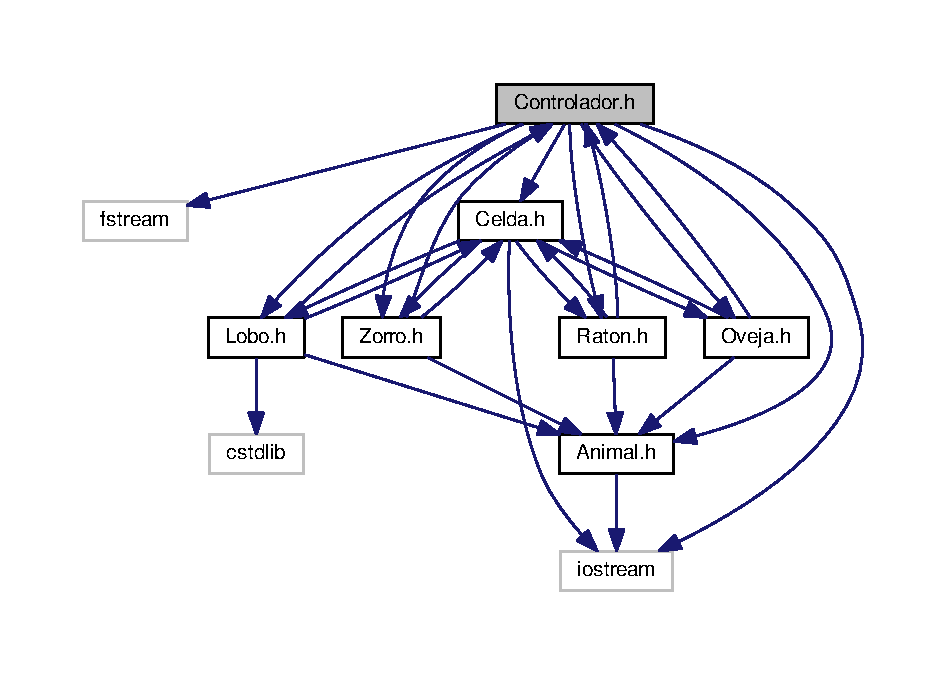
\includegraphics[width=350pt]{Controlador_8h__incl}
\end{center}
\end{figure}
This graph shows which files directly or indirectly include this file\+:
\nopagebreak
\begin{figure}[H]
\begin{center}
\leavevmode
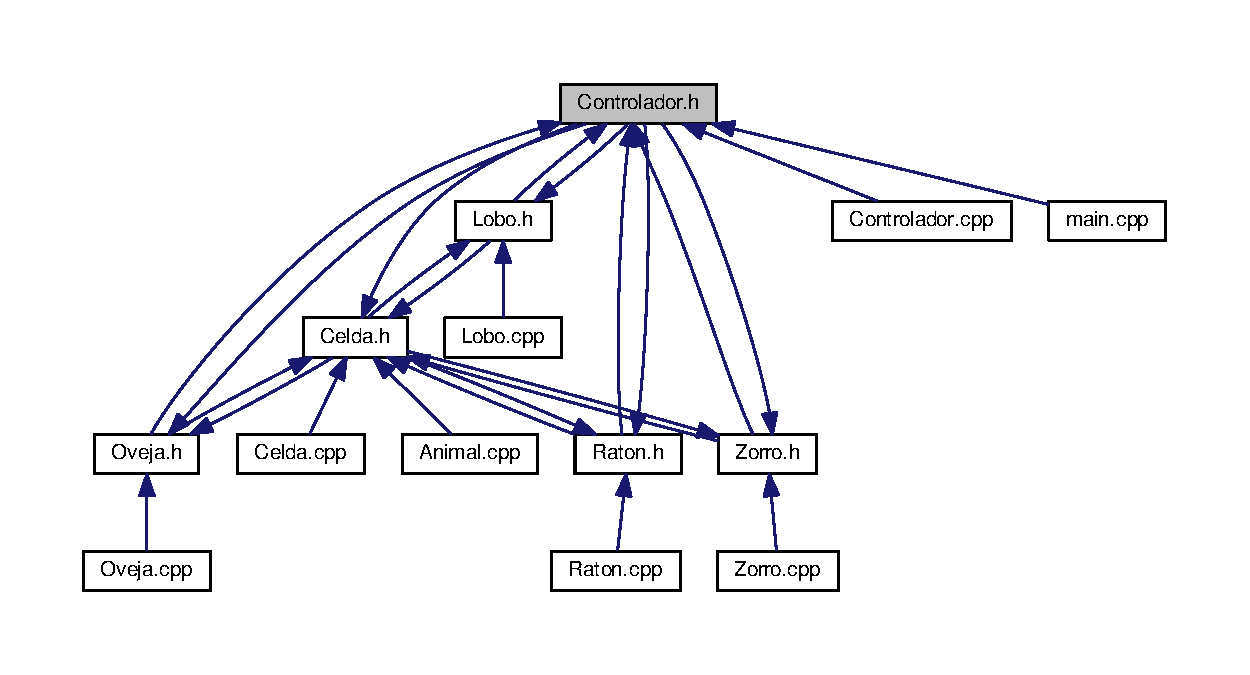
\includegraphics[width=240pt]{Controlador_8h__dep__incl}
\end{center}
\end{figure}
\subsection*{Data Structures}
\begin{DoxyCompactItemize}
\item 
class \hyperlink{classControlador}{Controlador}
\end{DoxyCompactItemize}
\subsection*{Functions}
\begin{DoxyCompactItemize}
\item 
{\footnotesize template$<$typename Data\+Type $>$ }\\void \hyperlink{Controlador_8h_aa4169f9f321bdec830a92aa0b9f9fe41}{print} (Data\+Type objeto)
\end{DoxyCompactItemize}


\subsection{Function Documentation}
\index{Controlador.\+h@{Controlador.\+h}!print@{print}}
\index{print@{print}!Controlador.\+h@{Controlador.\+h}}
\subsubsection[{\texorpdfstring{print(\+Data\+Type objeto)}{print(DataType objeto)}}]{\setlength{\rightskip}{0pt plus 5cm}template$<$typename Data\+Type $>$ void print (
\begin{DoxyParamCaption}
\item[{Data\+Type}]{objeto}
\end{DoxyParamCaption}
)}\hypertarget{Controlador_8h_aa4169f9f321bdec830a92aa0b9f9fe41}{}\label{Controlador_8h_aa4169f9f321bdec830a92aa0b9f9fe41}

\hypertarget{datos_8txt}{}\section{datos.\+txt File Reference}
\label{datos_8txt}\index{datos.\+txt@{datos.\+txt}}

\hypertarget{Lobo_8cpp}{}\section{Lobo.\+cpp File Reference}
\label{Lobo_8cpp}\index{Lobo.\+cpp@{Lobo.\+cpp}}


Clase \hyperlink{classLobo}{Lobo}.  


{\ttfamily \#include \char`\"{}Lobo.\+h\char`\"{}}\\*
Include dependency graph for Lobo.\+cpp\+:\nopagebreak
\begin{figure}[H]
\begin{center}
\leavevmode
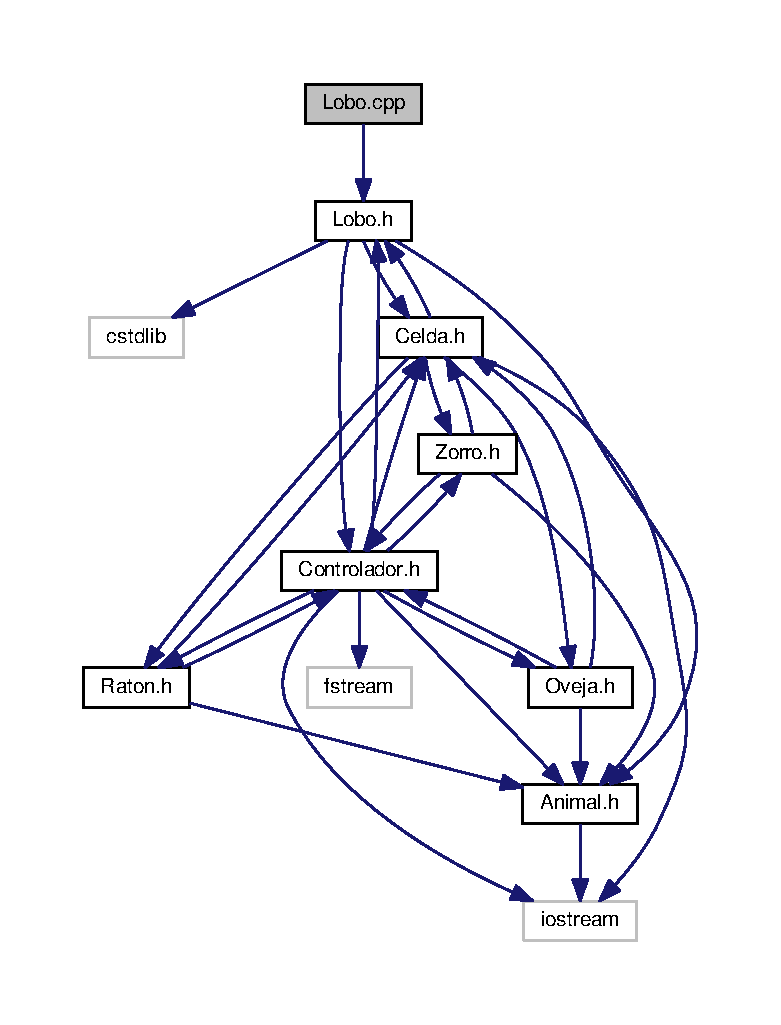
\includegraphics[width=350pt]{Lobo_8cpp__incl}
\end{center}
\end{figure}


\subsection{Detailed Description}
Clase \hyperlink{classLobo}{Lobo}. 

\begin{DoxyVersion}{Version}
1.\+0 
\end{DoxyVersion}
\begin{DoxyDate}{Date}
29/01/17 
\end{DoxyDate}
\begin{DoxyAuthor}{Author}
Luis Diego Fernandez, Daniel Jimenez  Juego de la vida 
\end{DoxyAuthor}

\hypertarget{Lobo_8h}{}\section{Lobo.\+h File Reference}
\label{Lobo_8h}\index{Lobo.\+h@{Lobo.\+h}}
{\ttfamily \#include $<$cstdlib$>$}\\*
{\ttfamily \#include \char`\"{}Animal.\+h\char`\"{}}\\*
Include dependency graph for Lobo.\+h\+:
\nopagebreak
\begin{figure}[H]
\begin{center}
\leavevmode
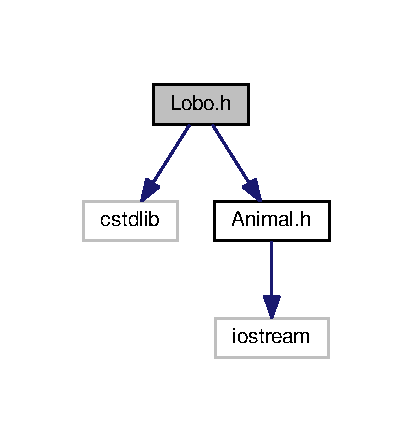
\includegraphics[width=198pt]{Lobo_8h__incl}
\end{center}
\end{figure}
This graph shows which files directly or indirectly include this file\+:
\nopagebreak
\begin{figure}[H]
\begin{center}
\leavevmode
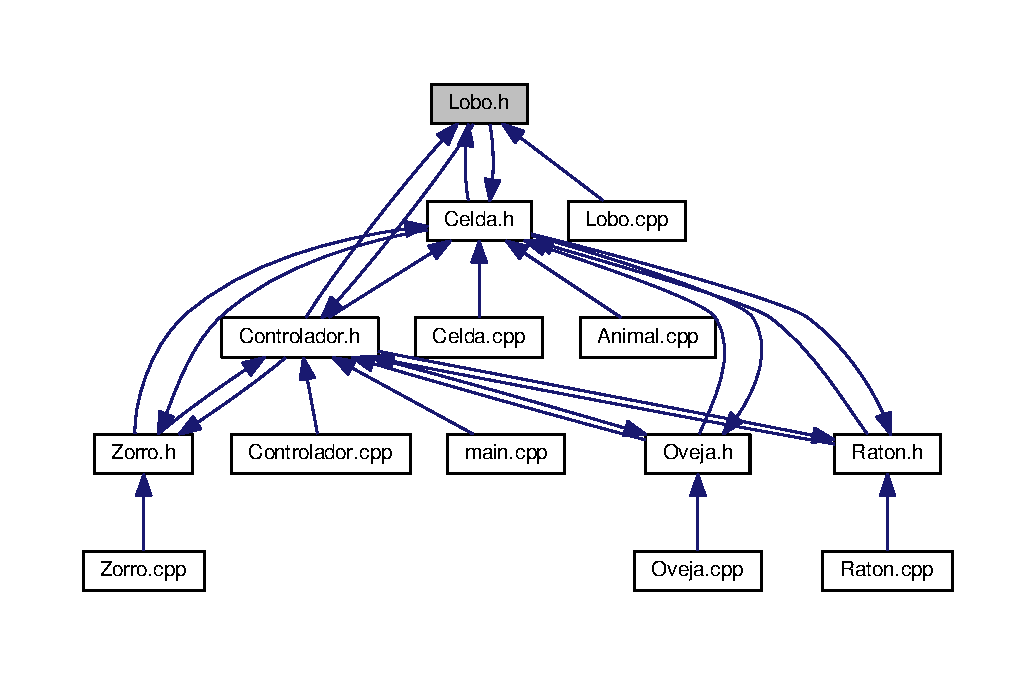
\includegraphics[width=350pt]{Lobo_8h__dep__incl}
\end{center}
\end{figure}
\subsection*{Data Structures}
\begin{DoxyCompactItemize}
\item 
class \hyperlink{classLobo}{Lobo}
\end{DoxyCompactItemize}

\hypertarget{main_8cpp}{}\section{main.\+cpp File Reference}
\label{main_8cpp}\index{main.\+cpp@{main.\+cpp}}
{\ttfamily \#include $<$stdlib.\+h$>$}\\*
{\ttfamily \#include \char`\"{}Controlador.\+h\char`\"{}}\\*
Include dependency graph for main.\+cpp\+:\nopagebreak
\begin{figure}[H]
\begin{center}
\leavevmode
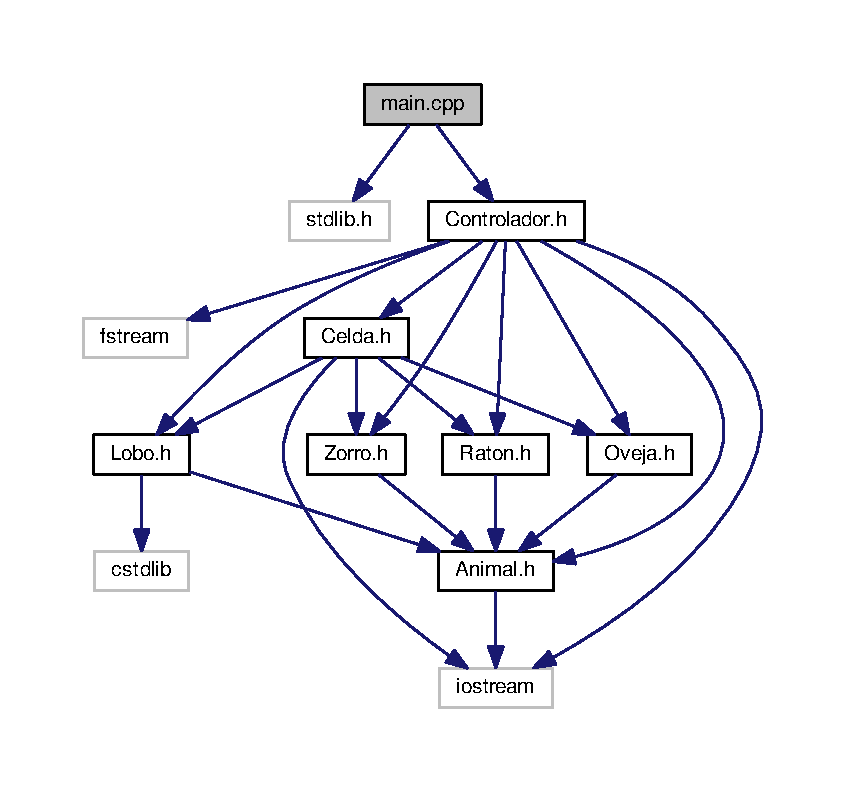
\includegraphics[width=350pt]{main_8cpp__incl}
\end{center}
\end{figure}
\subsection*{Functions}
\begin{DoxyCompactItemize}
\item 
int \hyperlink{main_8cpp_a0ddf1224851353fc92bfbff6f499fa97}{main} (int argc, char $\ast$argv\mbox{[}$\,$\mbox{]})
\end{DoxyCompactItemize}


\subsection{Function Documentation}
\index{main.\+cpp@{main.\+cpp}!main@{main}}
\index{main@{main}!main.\+cpp@{main.\+cpp}}
\subsubsection[{\texorpdfstring{main(int argc, char $\ast$argv[])}{main(int argc, char *argv[])}}]{\setlength{\rightskip}{0pt plus 5cm}int main (
\begin{DoxyParamCaption}
\item[{int}]{argc, }
\item[{char $\ast$}]{argv\mbox{[}$\,$\mbox{]}}
\end{DoxyParamCaption}
)}\hypertarget{main_8cpp_a0ddf1224851353fc92bfbff6f499fa97}{}\label{main_8cpp_a0ddf1224851353fc92bfbff6f499fa97}

\hypertarget{Oveja_8cpp}{}\section{Oveja.\+cpp File Reference}
\label{Oveja_8cpp}\index{Oveja.\+cpp@{Oveja.\+cpp}}


Clase \hyperlink{classOveja}{Oveja}.  


{\ttfamily \#include \char`\"{}Oveja.\+h\char`\"{}}\\*
Include dependency graph for Oveja.\+cpp\+:\nopagebreak
\begin{figure}[H]
\begin{center}
\leavevmode
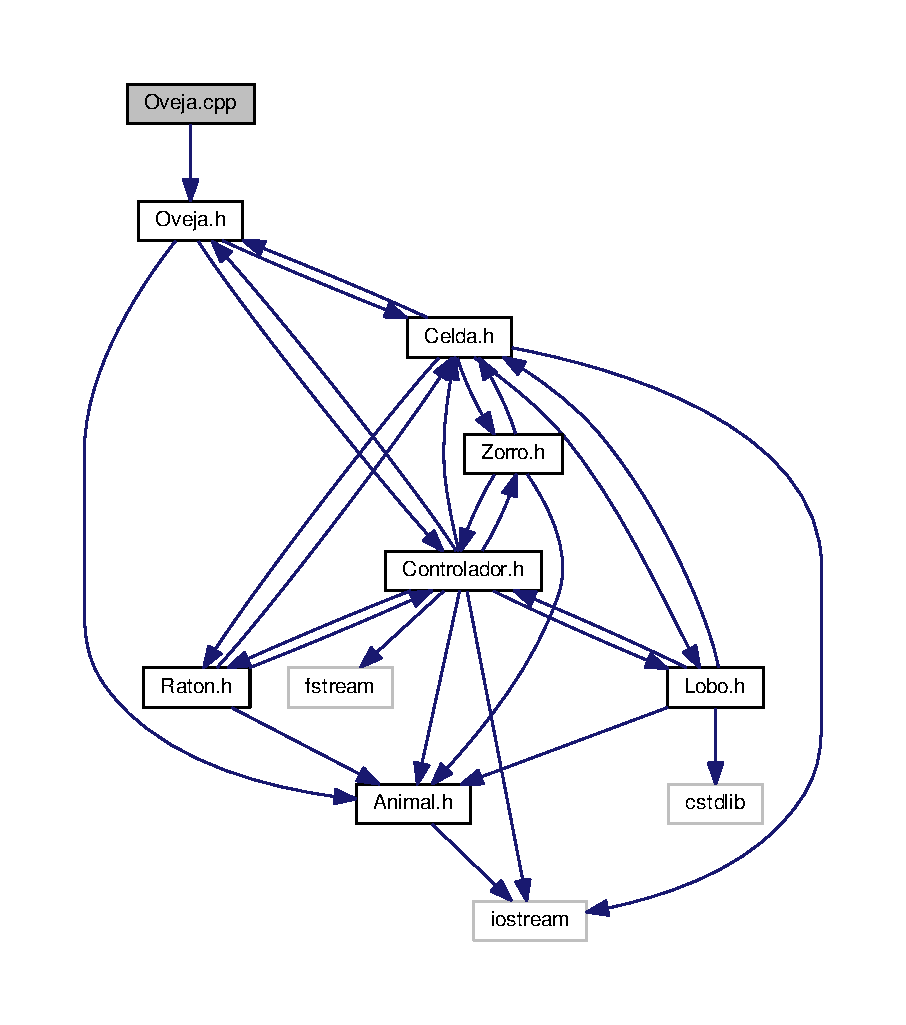
\includegraphics[width=350pt]{Oveja_8cpp__incl}
\end{center}
\end{figure}


\subsection{Detailed Description}
Clase \hyperlink{classOveja}{Oveja}. 

\begin{DoxyVersion}{Version}
1.\+0 
\end{DoxyVersion}
\begin{DoxyDate}{Date}
29/01/17 
\end{DoxyDate}
\begin{DoxyAuthor}{Author}
Luis Diego Fernandez, Daniel Jimenez  Juego de la vida 
\end{DoxyAuthor}

\hypertarget{Oveja_8h}{}\section{Oveja.\+h File Reference}
\label{Oveja_8h}\index{Oveja.\+h@{Oveja.\+h}}
{\ttfamily \#include \char`\"{}Animal.\+h\char`\"{}}\\*
Include dependency graph for Oveja.\+h\+:
\nopagebreak
\begin{figure}[H]
\begin{center}
\leavevmode
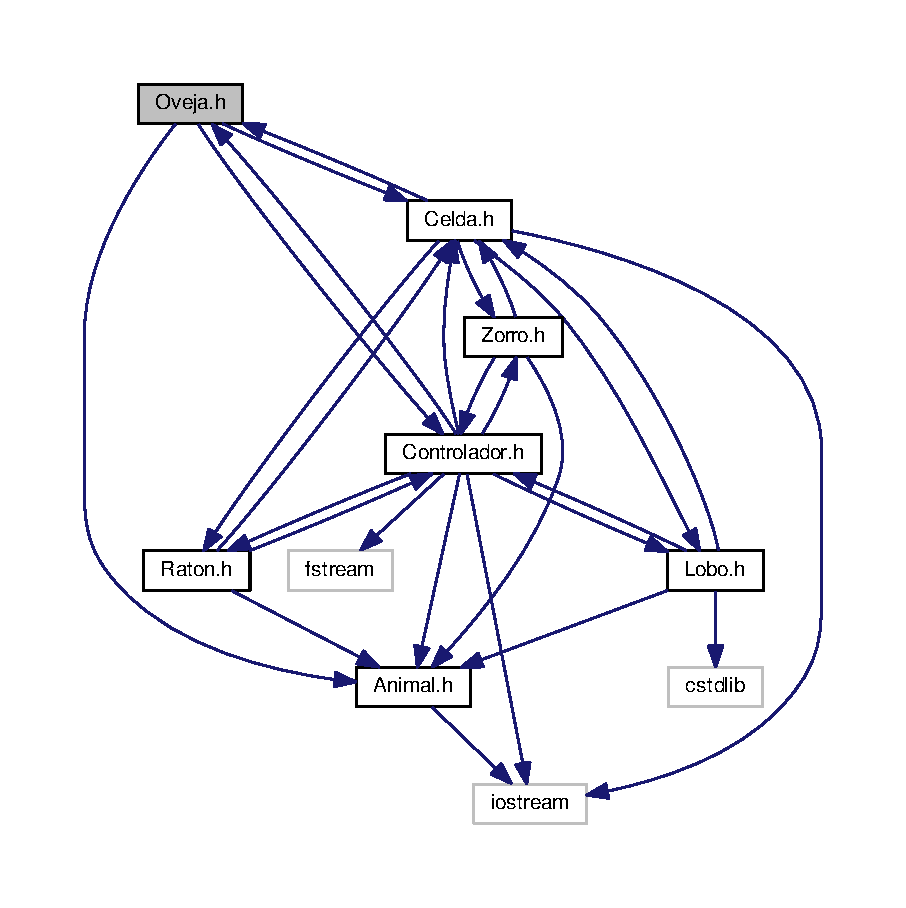
\includegraphics[width=135pt]{Oveja_8h__incl}
\end{center}
\end{figure}
This graph shows which files directly or indirectly include this file\+:
\nopagebreak
\begin{figure}[H]
\begin{center}
\leavevmode
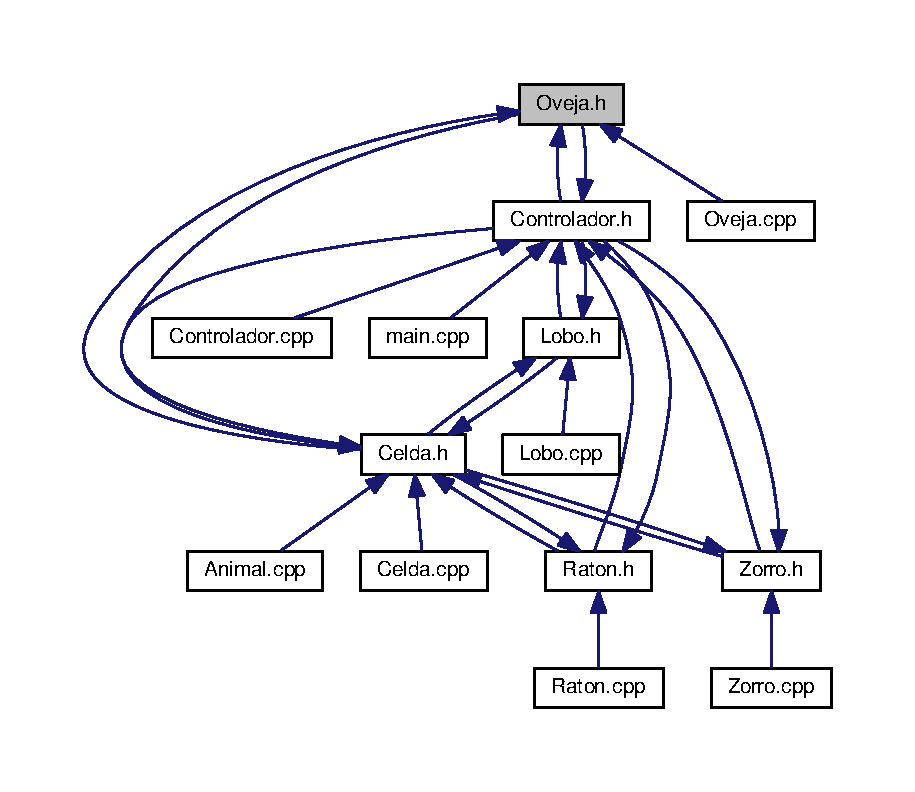
\includegraphics[width=350pt]{Oveja_8h__dep__incl}
\end{center}
\end{figure}
\subsection*{Data Structures}
\begin{DoxyCompactItemize}
\item 
class \hyperlink{classOveja}{Oveja}
\end{DoxyCompactItemize}

\hypertarget{Raton_8cpp}{}\section{Raton.\+cpp File Reference}
\label{Raton_8cpp}\index{Raton.\+cpp@{Raton.\+cpp}}


Clase \hyperlink{classRaton}{Raton}.  


{\ttfamily \#include \char`\"{}Raton.\+h\char`\"{}}\\*
Include dependency graph for Raton.\+cpp\+:\nopagebreak
\begin{figure}[H]
\begin{center}
\leavevmode
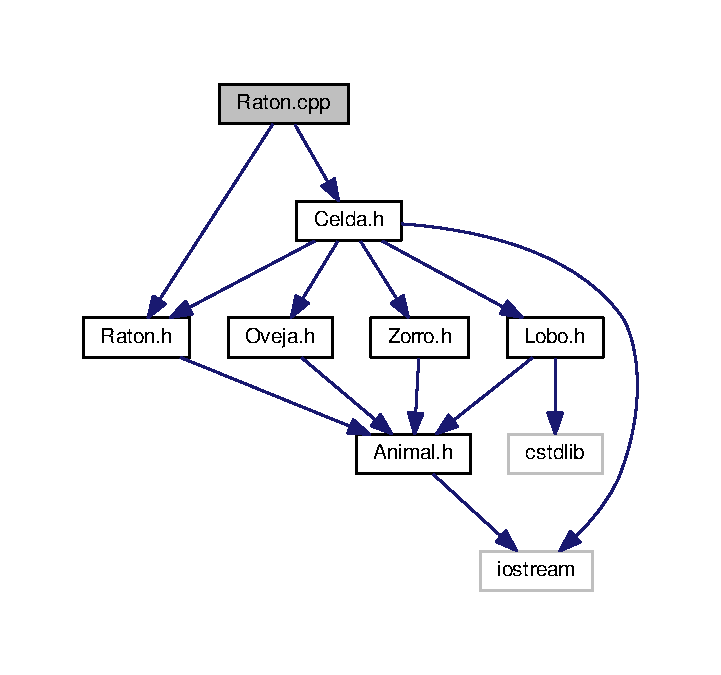
\includegraphics[width=350pt]{Raton_8cpp__incl}
\end{center}
\end{figure}


\subsection{Detailed Description}
Clase \hyperlink{classRaton}{Raton}. 

\begin{DoxyVersion}{Version}
1.\+0 
\end{DoxyVersion}
\begin{DoxyDate}{Date}
29/01/17 
\end{DoxyDate}
\begin{DoxyAuthor}{Author}
Luis Diego Fernandez, Daniel Jimenez  Juego de la vida 
\end{DoxyAuthor}

\hypertarget{Raton_8h}{}\section{Raton.\+h File Reference}
\label{Raton_8h}\index{Raton.\+h@{Raton.\+h}}
{\ttfamily \#include \char`\"{}Animal.\+h\char`\"{}}\\*
Include dependency graph for Raton.\+h\+:
\nopagebreak
\begin{figure}[H]
\begin{center}
\leavevmode
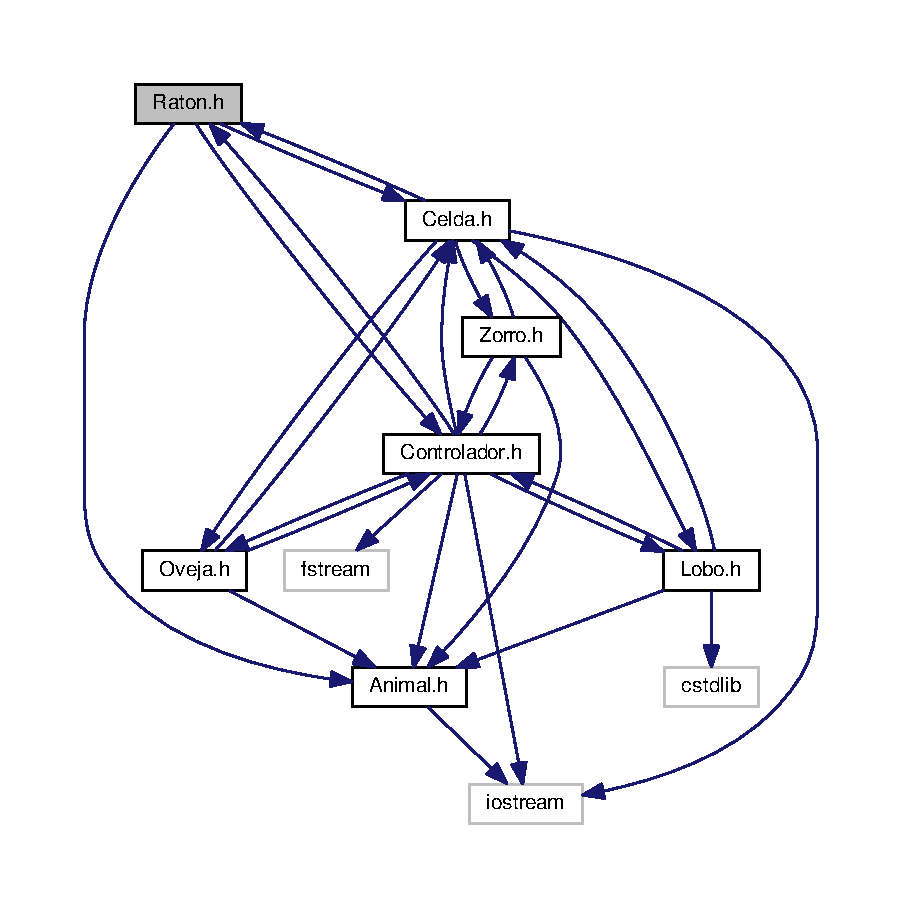
\includegraphics[width=135pt]{Raton_8h__incl}
\end{center}
\end{figure}
This graph shows which files directly or indirectly include this file\+:
\nopagebreak
\begin{figure}[H]
\begin{center}
\leavevmode
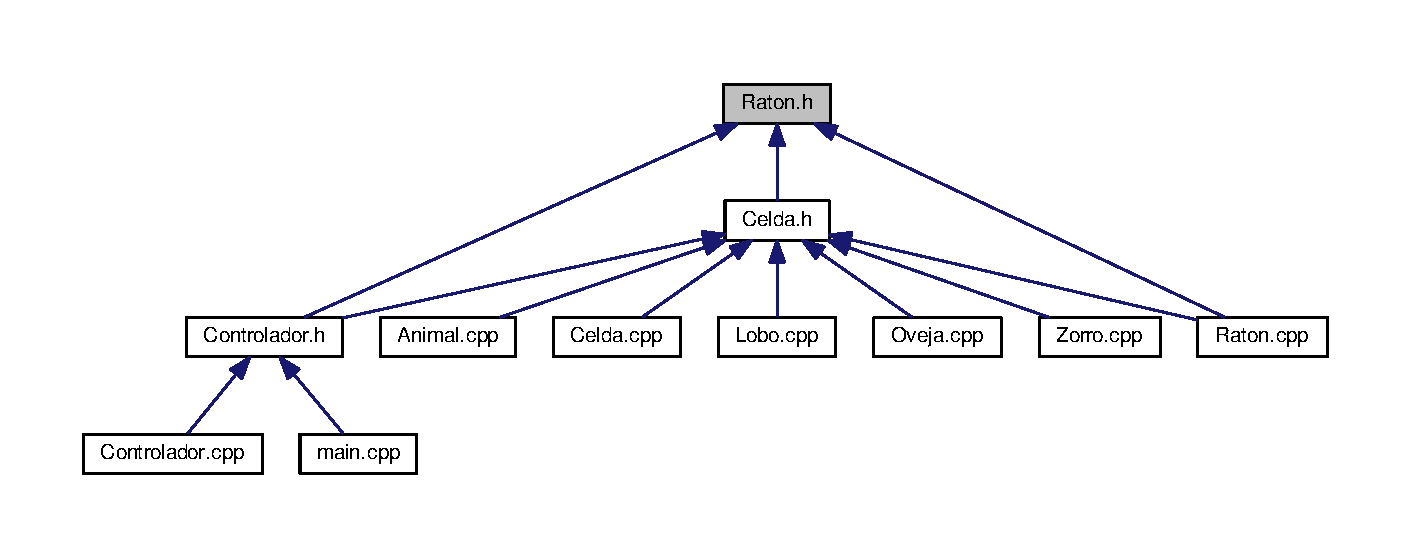
\includegraphics[width=350pt]{Raton_8h__dep__incl}
\end{center}
\end{figure}
\subsection*{Data Structures}
\begin{DoxyCompactItemize}
\item 
class \hyperlink{classRaton}{Raton}
\end{DoxyCompactItemize}

\hypertarget{Zorro_8cpp}{}\section{Zorro.\+cpp File Reference}
\label{Zorro_8cpp}\index{Zorro.\+cpp@{Zorro.\+cpp}}


Clase \hyperlink{classZorro}{Zorro}.  


{\ttfamily \#include \char`\"{}Zorro.\+h\char`\"{}}\\*
{\ttfamily \#include \char`\"{}Celda.\+h\char`\"{}}\\*
Include dependency graph for Zorro.\+cpp\+:
\nopagebreak
\begin{figure}[H]
\begin{center}
\leavevmode
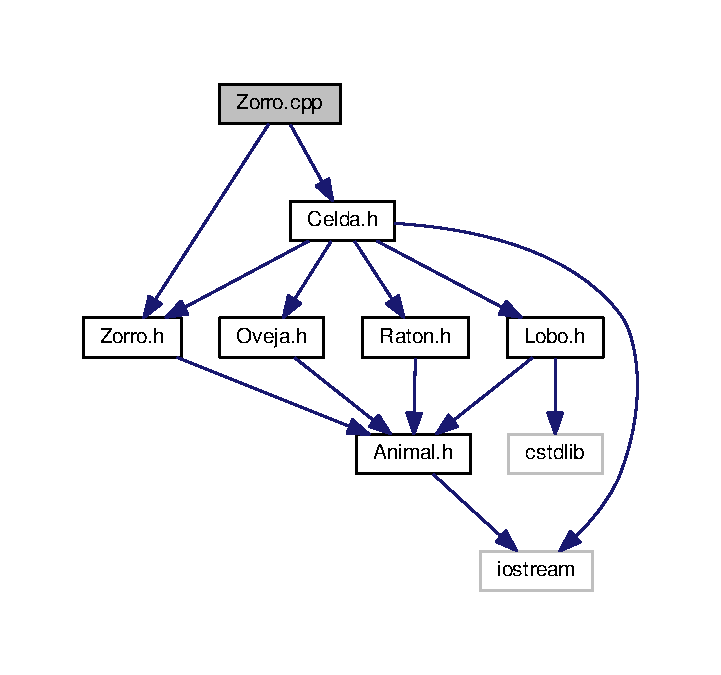
\includegraphics[width=346pt]{Zorro_8cpp__incl}
\end{center}
\end{figure}


\subsection{Detailed Description}
Clase \hyperlink{classZorro}{Zorro}. 

\begin{DoxyVersion}{Version}
1.\+0 
\end{DoxyVersion}
\begin{DoxyDate}{Date}
29/01/17 
\end{DoxyDate}
\begin{DoxyAuthor}{Author}
Luis Diego Fernandez, Daniel Jimenez  Juego de la vida 
\end{DoxyAuthor}

\hypertarget{Zorro_8h}{}\section{Zorro.\+h File Reference}
\label{Zorro_8h}\index{Zorro.\+h@{Zorro.\+h}}
{\ttfamily \#include \char`\"{}Animal.\+h\char`\"{}}\\*
Include dependency graph for Zorro.\+h\+:
\nopagebreak
\begin{figure}[H]
\begin{center}
\leavevmode
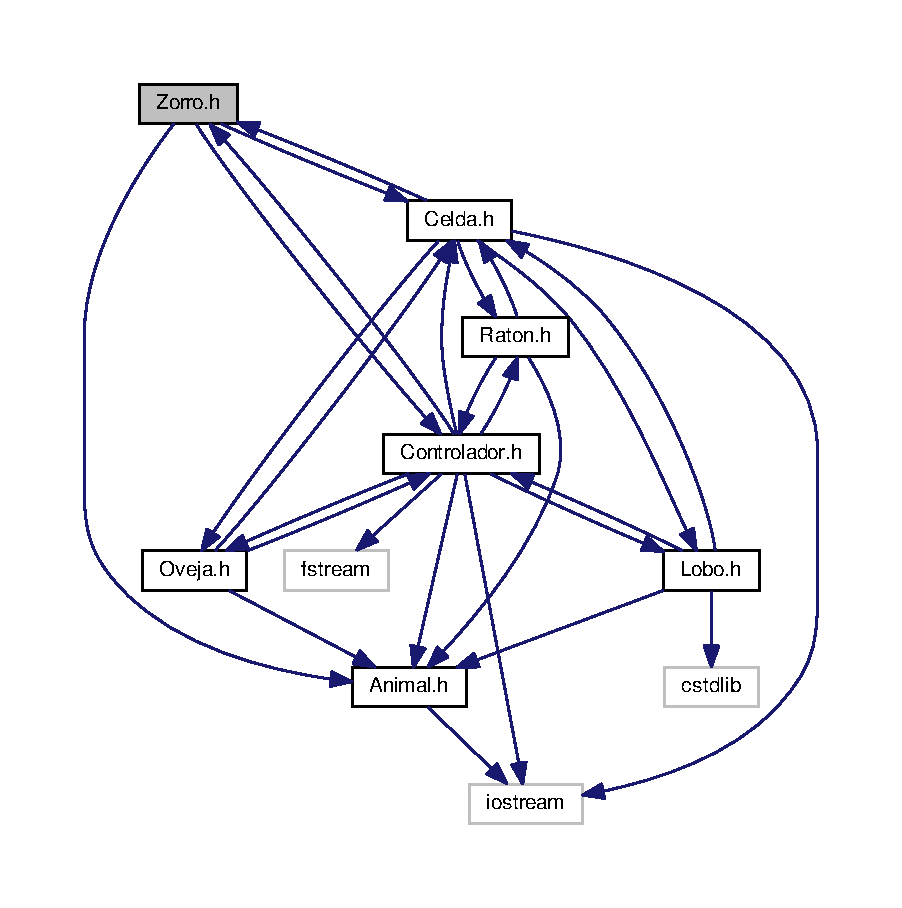
\includegraphics[width=135pt]{Zorro_8h__incl}
\end{center}
\end{figure}
This graph shows which files directly or indirectly include this file\+:
\nopagebreak
\begin{figure}[H]
\begin{center}
\leavevmode
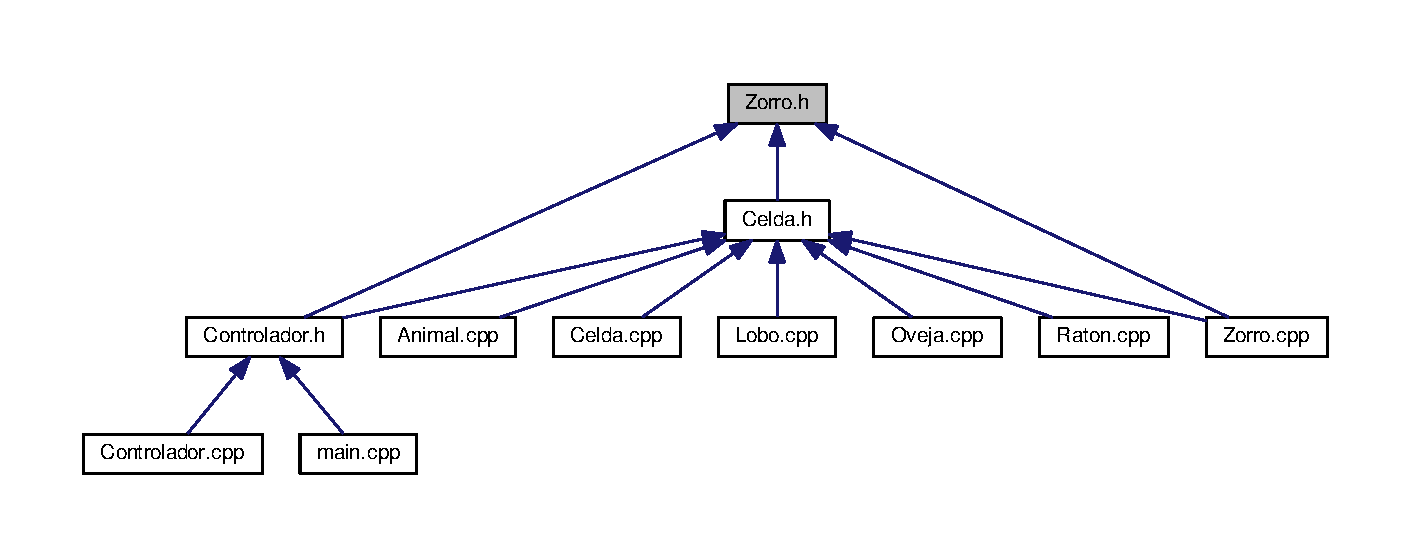
\includegraphics[width=350pt]{Zorro_8h__dep__incl}
\end{center}
\end{figure}
\subsection*{Data Structures}
\begin{DoxyCompactItemize}
\item 
class \hyperlink{classZorro}{Zorro}
\end{DoxyCompactItemize}

%--- End generated contents ---

% Index
\backmatter
\newpage
\phantomsection
\clearemptydoublepage
\addcontentsline{toc}{chapter}{Index}
\printindex

\end{document}
